\batchmode
\documentclass[twoside]{book}

% Packages required by doxygen
\usepackage{fixltx2e}
\usepackage{calc}
\usepackage{doxygen}
\usepackage[export]{adjustbox} % also loads graphicx
\usepackage{graphicx}
\usepackage[utf8]{inputenc}
\usepackage{makeidx}
\usepackage{multicol}
\usepackage{multirow}
\PassOptionsToPackage{warn}{textcomp}
\usepackage{textcomp}
\usepackage[nointegrals]{wasysym}
\usepackage[table]{xcolor}

% Font selection
\usepackage[T1]{fontenc}
\usepackage[scaled=.90]{helvet}
\usepackage{courier}
\usepackage{amssymb}
\usepackage{sectsty}
\renewcommand{\familydefault}{\sfdefault}
\allsectionsfont{%
  \fontseries{bc}\selectfont%
  \color{darkgray}%
}
\renewcommand{\DoxyLabelFont}{%
  \fontseries{bc}\selectfont%
  \color{darkgray}%
}
\newcommand{\+}{\discretionary{\mbox{\scriptsize$\hookleftarrow$}}{}{}}

% Page & text layout
\usepackage{geometry}
\geometry{%
  a4paper,%
  top=2.5cm,%
  bottom=2.5cm,%
  left=2.5cm,%
  right=2.5cm%
}
\tolerance=750
\hfuzz=15pt
\hbadness=750
\setlength{\emergencystretch}{15pt}
\setlength{\parindent}{0cm}
\setlength{\parskip}{3ex plus 2ex minus 2ex}
\makeatletter
\renewcommand{\paragraph}{%
  \@startsection{paragraph}{4}{0ex}{-1.0ex}{1.0ex}{%
    \normalfont\normalsize\bfseries\SS@parafont%
  }%
}
\renewcommand{\subparagraph}{%
  \@startsection{subparagraph}{5}{0ex}{-1.0ex}{1.0ex}{%
    \normalfont\normalsize\bfseries\SS@subparafont%
  }%
}
\makeatother

% Headers & footers
\usepackage{fancyhdr}
\pagestyle{fancyplain}
\fancyhead[LE]{\fancyplain{}{\bfseries\thepage}}
\fancyhead[CE]{\fancyplain{}{}}
\fancyhead[RE]{\fancyplain{}{\bfseries\leftmark}}
\fancyhead[LO]{\fancyplain{}{\bfseries\rightmark}}
\fancyhead[CO]{\fancyplain{}{}}
\fancyhead[RO]{\fancyplain{}{\bfseries\thepage}}
\fancyfoot[LE]{\fancyplain{}{}}
\fancyfoot[CE]{\fancyplain{}{}}
\fancyfoot[RE]{\fancyplain{}{\bfseries\scriptsize Generated by Doxygen }}
\fancyfoot[LO]{\fancyplain{}{\bfseries\scriptsize Generated by Doxygen }}
\fancyfoot[CO]{\fancyplain{}{}}
\fancyfoot[RO]{\fancyplain{}{}}
\renewcommand{\footrulewidth}{0.4pt}
\renewcommand{\chaptermark}[1]{%
  \markboth{#1}{}%
}
\renewcommand{\sectionmark}[1]{%
  \markright{\thesection\ #1}%
}

% Indices & bibliography
\usepackage{natbib}
\usepackage[titles]{tocloft}
\setcounter{tocdepth}{3}
\setcounter{secnumdepth}{5}
\makeindex

% Hyperlinks (required, but should be loaded last)
\usepackage{ifpdf}
\ifpdf
  \usepackage[pdftex,pagebackref=true]{hyperref}
\else
  \usepackage[ps2pdf,pagebackref=true]{hyperref}
\fi
\hypersetup{%
  colorlinks=true,%
  linkcolor=blue,%
  citecolor=blue,%
  unicode%
}

% Custom commands
\newcommand{\clearemptydoublepage}{%
  \newpage{\pagestyle{empty}\cleardoublepage}%
}

\usepackage{caption}
\captionsetup{labelsep=space,justification=centering,font={bf},singlelinecheck=off,skip=4pt,position=top}

%===== C O N T E N T S =====

\begin{document}

% Titlepage & ToC
\hypersetup{pageanchor=false,
             bookmarksnumbered=true,
             pdfencoding=unicode
            }
\pagenumbering{alph}
\pagenumbering{arabic}
\hypersetup{pageanchor=true}

%--- Begin generated contents ---
\chapter{Motion of an elliptical particle in shear flow\+: Jeffery orbits}
\label{index}\hypertarget{index}{}\hypertarget{index_q}{}\section{A few quick questions...}\label{index_q}
Since {\ttfamily oomph-\/lib} is developed as open-\/source software, any evidence that the code is being downloaded and used is very helpful for us as it helps to justify our continued work on this project.

We would therefore be extremely grateful if you could provide the information requested in the form below. Pressing the \char`\"{}submit\char`\"{} button will get you to the actual download page.

{\bfseries Note\+:} 
\begin{DoxyItemize}
\item All information will be treated as confidential. 
\item If you provide your email address and check the appropriate box we will add you to our mailing list to inform you of upgrades and bug fixes to the code. Rest assured that the mailing list is {\bfseries very low volume} -- we have better things to do than to bombard you with email. 
\item If you still feel reluctant to provide any of the information requested, feel free to enter some dummy input. The form will check that {\bfseries some} information has been entered but entering your name as \char`\"{}\+Joe Cool\char`\"{} is perfectly acceptable -- this is to discourage people from not providing the information simply because they are too lazy to type... 
\end{DoxyItemize}



 







 

 \hypertarget{index_pdf}{}\section{P\+D\+F file}\label{index_pdf}
A \href{../latex/refman.pdf}{\tt pdf version} of this document is available. \end{document}

\chapter{Namespace Index}
\section{Namespace List}
Here is a list of all namespaces with brief descriptions\+:\begin{DoxyCompactList}
\item\contentsline{section}{\hyperlink{namespaceGlobal__Physical__Variables}{Global\+\_\+\+Physical\+\_\+\+Variables} \\*Global variables that represent physical properties }{\pageref{namespaceGlobal__Physical__Variables}}{}
\item\contentsline{section}{\hyperlink{namespaceoomph}{oomph} }{\pageref{namespaceoomph}}{}
\item\contentsline{section}{\hyperlink{namespacePhysical__Variables}{Physical\+\_\+\+Variables} \\*Namespace for the solution of 2D linear shell equation }{\pageref{namespacePhysical__Variables}}{}
\end{DoxyCompactList}

\chapter{Hierarchical Index}
\section{Class Hierarchy}
This inheritance list is sorted roughly, but not completely, alphabetically\+:\begin{DoxyCompactList}
\item Problem\begin{DoxyCompactList}
\item \contentsline{section}{Unstructured\+Solid\+Problem$<$ E\+L\+E\+M\+E\+NT $>$}{\pageref{classUnstructuredSolidProblem}}{}
\end{DoxyCompactList}
\end{DoxyCompactList}

\chapter{Class Index}
\section{Class List}
Here are the classes, structs, unions and interfaces with brief descriptions\+:\begin{DoxyCompactList}
\item\contentsline{section}{\hyperlink{classPMLProblem}{P\+M\+L\+Problem$<$ E\+L\+E\+M\+E\+N\+T $>$} }{\pageref{classPMLProblem}}{}
\item\contentsline{section}{\hyperlink{classGlobalParameters_1_1TestPMLMapping}{Global\+Parameters\+::\+Test\+P\+M\+L\+Mapping} }{\pageref{classGlobalParameters_1_1TestPMLMapping}}{}
\end{DoxyCompactList}

\chapter{File Index}
\section{File List}
Here is a list of all files with brief descriptions\+:\begin{DoxyCompactList}
\item\contentsline{section}{\hyperlink{jeffery__orbit_8cc}{jeffery\+\_\+orbit.\+cc} }{\pageref{jeffery__orbit_8cc}}{}
\item\contentsline{section}{\hyperlink{jeffery__orbit_8txt__doxygenified_8h}{jeffery\+\_\+orbit.\+txt\+\_\+doxygenified.\+h} }{\pageref{jeffery__orbit_8txt__doxygenified_8h}}{}
\item\contentsline{section}{\hyperlink{my__taylor__hood__elements_8h}{my\+\_\+taylor\+\_\+hood\+\_\+elements.\+h} }{\pageref{my__taylor__hood__elements_8h}}{}
\end{DoxyCompactList}

\chapter{Namespace Documentation}
\hypertarget{namespaceJeffery__Solution}{}\section{Jeffery\+\_\+\+Solution Namespace Reference}
\label{namespaceJeffery__Solution}\index{Jeffery\+\_\+\+Solution@{Jeffery\+\_\+\+Solution}}
\subsection*{Functions}
\begin{DoxyCompactItemize}
\item 
double \hyperlink{namespaceJeffery__Solution_a6a47b12e9a89f545c7467fae2e6a4350}{null} (const double \&t)
\begin{DoxyCompactList}\small\item\em Null function. \end{DoxyCompactList}\item 
double \hyperlink{namespaceJeffery__Solution_ad3bd18834ecba370674e34242f8125c1}{angle} (const double \&t)
\begin{DoxyCompactList}\small\item\em Angular position as a function of time t. \end{DoxyCompactList}\item 
double \hyperlink{namespaceJeffery__Solution_acf35d547e7d28609a17c66c9a191090b}{velocity} (const double \&t)
\begin{DoxyCompactList}\small\item\em Angular velocity as function of time t. \end{DoxyCompactList}\item 
double \hyperlink{namespaceJeffery__Solution_afe09bdca1fe833f94f510e206d5df08c}{acceleration} (const double \&t)
\begin{DoxyCompactList}\small\item\em Angular acceleration as a function of time t (should always be zero) \end{DoxyCompactList}\end{DoxyCompactItemize}


\subsection{Detailed Description}
Exact solution for the rotation of an ellipse in unbounded shear flow as computed by Jeffery (1922) 

\subsection{Function Documentation}
\mbox{\Hypertarget{namespaceJeffery__Solution_afe09bdca1fe833f94f510e206d5df08c}\label{namespaceJeffery__Solution_afe09bdca1fe833f94f510e206d5df08c}} 
\index{Jeffery\+\_\+\+Solution@{Jeffery\+\_\+\+Solution}!acceleration@{acceleration}}
\index{acceleration@{acceleration}!Jeffery\+\_\+\+Solution@{Jeffery\+\_\+\+Solution}}
\subsubsection{\texorpdfstring{acceleration()}{acceleration()}}
{\footnotesize\ttfamily double Jeffery\+\_\+\+Solution\+::acceleration (\begin{DoxyParamCaption}\item[{const double \&}]{t }\end{DoxyParamCaption})}



Angular acceleration as a function of time t (should always be zero) 



Definition at line 124 of file jeffery\+\_\+orbit.\+cc.



References Problem\+\_\+\+Parameter\+::A, angle(), and velocity().



Referenced by Unstructured\+Immersed\+Ellipse\+Problem$<$ E\+L\+E\+M\+E\+N\+T $>$\+::output\+\_\+exact\+\_\+solution().

\mbox{\Hypertarget{namespaceJeffery__Solution_ad3bd18834ecba370674e34242f8125c1}\label{namespaceJeffery__Solution_ad3bd18834ecba370674e34242f8125c1}} 
\index{Jeffery\+\_\+\+Solution@{Jeffery\+\_\+\+Solution}!angle@{angle}}
\index{angle@{angle}!Jeffery\+\_\+\+Solution@{Jeffery\+\_\+\+Solution}}
\subsubsection{\texorpdfstring{angle()}{angle()}}
{\footnotesize\ttfamily double Jeffery\+\_\+\+Solution\+::angle (\begin{DoxyParamCaption}\item[{const double \&}]{t }\end{DoxyParamCaption})}



Angular position as a function of time t. 



Definition at line 102 of file jeffery\+\_\+orbit.\+cc.



References Problem\+\_\+\+Parameter\+::A, and Problem\+\_\+\+Parameter\+::B.



Referenced by acceleration(), Unstructured\+Immersed\+Ellipse\+Problem$<$ E\+L\+E\+M\+E\+N\+T $>$\+::output\+\_\+exact\+\_\+solution(), and velocity().

\mbox{\Hypertarget{namespaceJeffery__Solution_a6a47b12e9a89f545c7467fae2e6a4350}\label{namespaceJeffery__Solution_a6a47b12e9a89f545c7467fae2e6a4350}} 
\index{Jeffery\+\_\+\+Solution@{Jeffery\+\_\+\+Solution}!null@{null}}
\index{null@{null}!Jeffery\+\_\+\+Solution@{Jeffery\+\_\+\+Solution}}
\subsubsection{\texorpdfstring{null()}{null()}}
{\footnotesize\ttfamily double Jeffery\+\_\+\+Solution\+::null (\begin{DoxyParamCaption}\item[{const double \&}]{t }\end{DoxyParamCaption})}



Null function. 



Definition at line 99 of file jeffery\+\_\+orbit.\+cc.

\mbox{\Hypertarget{namespaceJeffery__Solution_acf35d547e7d28609a17c66c9a191090b}\label{namespaceJeffery__Solution_acf35d547e7d28609a17c66c9a191090b}} 
\index{Jeffery\+\_\+\+Solution@{Jeffery\+\_\+\+Solution}!velocity@{velocity}}
\index{velocity@{velocity}!Jeffery\+\_\+\+Solution@{Jeffery\+\_\+\+Solution}}
\subsubsection{\texorpdfstring{velocity()}{velocity()}}
{\footnotesize\ttfamily double Jeffery\+\_\+\+Solution\+::velocity (\begin{DoxyParamCaption}\item[{const double \&}]{t }\end{DoxyParamCaption})}



Angular velocity as function of time t. 



Definition at line 111 of file jeffery\+\_\+orbit.\+cc.



References Problem\+\_\+\+Parameter\+::A, angle(), and Problem\+\_\+\+Parameter\+::B.



Referenced by acceleration(), and Unstructured\+Immersed\+Ellipse\+Problem$<$ E\+L\+E\+M\+E\+N\+T $>$\+::output\+\_\+exact\+\_\+solution().


\hypertarget{namespaceoomph}{}\section{oomph Namespace Reference}
\label{namespaceoomph}\index{oomph@{oomph}}
\subsection*{Classes}
\begin{DoxyCompactItemize}
\item 
class \hyperlink{classoomph_1_1BellShellElement}{Bell\+Shell\+Element}
\begin{DoxyCompactList}\small\item\em \hyperlink{classoomph_1_1BellShellElement}{Bell\+Shell\+Element} elements are with subparametric interpolation for the function. \end{DoxyCompactList}\item 
class \hyperlink{classoomph_1_1FaceGeometry_3_01BellShellElement_3_01DIM_00_01NNODE__1D_01_4_01_4}{Face\+Geometry$<$ Bell\+Shell\+Element$<$ D\+I\+M, N\+N\+O\+D\+E\+\_\+1\+D $>$ $>$}
\item 
class \hyperlink{classoomph_1_1MyShellEquations}{My\+Shell\+Equations}
\item 
class \hyperlink{classoomph_1_1Plate}{Plate}
\begin{DoxyCompactList}\small\item\em Elliptical tube with half axes a and b. \end{DoxyCompactList}\end{DoxyCompactItemize}

\hypertarget{namespaceProblem__Parameter}{}\section{Problem\+\_\+\+Parameter Namespace Reference}
\label{namespaceProblem__Parameter}\index{Problem\+\_\+\+Parameter@{Problem\+\_\+\+Parameter}}


Namespace for Problem Parameters.  


\subsection*{Variables}
\begin{DoxyCompactItemize}
\item 
double \hyperlink{namespaceProblem__Parameter_acc656299287d4d9a8374c2c501750b4f}{Re} =1.\+0
\begin{DoxyCompactList}\small\item\em Reynolds number. \end{DoxyCompactList}\item 
double \hyperlink{namespaceProblem__Parameter_a8d9b76e390569bac0095bd0952281a30}{St} = 1.\+0
\begin{DoxyCompactList}\small\item\em Strouhal number. \end{DoxyCompactList}\item 
double \hyperlink{namespaceProblem__Parameter_a7fcb9a415485247d626190923235be2a}{Density\+\_\+ratio} = 1.\+0
\begin{DoxyCompactList}\small\item\em Density ratio (Solid density / Fluid density) \end{DoxyCompactList}\item 
double \hyperlink{namespaceProblem__Parameter_a23071148de0fea3597c2a7eb848320b6}{A} = 0.\+25
\begin{DoxyCompactList}\small\item\em Initial axis of the elliptical solid in x-\/direction. \end{DoxyCompactList}\item 
double \hyperlink{namespaceProblem__Parameter_ac2362a46222574a21338a113e2bee27e}{B} = 0.\+5
\item 
double \hyperlink{namespaceProblem__Parameter_abec2e733c8f2d3c18ebc702b3f80cc17}{Nu} =0.\+3
\begin{DoxyCompactList}\small\item\em Pseudo-\/solid (mesh) Poisson ratio. \end{DoxyCompactList}\item 
double \hyperlink{namespaceProblem__Parameter_a20ea33c391abd96d43f79913377c1e12}{Lambda\+\_\+sq} =0.\+0
\begin{DoxyCompactList}\small\item\em Pseudo-\/solid (mesh) \char`\"{}density\char`\"{} Set to zero because we don\textquotesingle{}t want inertia in the node update! \end{DoxyCompactList}\item 
Constitutive\+Law $\ast$ \hyperlink{namespaceProblem__Parameter_a9852a6077458693983628319d429f11f}{Constitutive\+\_\+law\+\_\+pt}
\begin{DoxyCompactList}\small\item\em Constitutive law used to determine the mesh deformation. \end{DoxyCompactList}\end{DoxyCompactItemize}


\subsection{Detailed Description}
Namespace for Problem Parameters. 

\subsection{Variable Documentation}
\mbox{\Hypertarget{namespaceProblem__Parameter_a23071148de0fea3597c2a7eb848320b6}\label{namespaceProblem__Parameter_a23071148de0fea3597c2a7eb848320b6}} 
\index{Problem\+\_\+\+Parameter@{Problem\+\_\+\+Parameter}!A@{A}}
\index{A@{A}!Problem\+\_\+\+Parameter@{Problem\+\_\+\+Parameter}}
\subsubsection{\texorpdfstring{A}{A}}
{\footnotesize\ttfamily double Problem\+\_\+\+Parameter\+::A = 0.\+25}



Initial axis of the elliptical solid in x-\/direction. 



Definition at line 72 of file jeffery\+\_\+orbit.\+cc.



Referenced by Jeffery\+\_\+\+Solution\+::acceleration(), Jeffery\+\_\+\+Solution\+::angle(), Unstructured\+Immersed\+Ellipse\+Problem$<$ E\+L\+E\+M\+E\+N\+T $>$\+::\+Unstructured\+Immersed\+Ellipse\+Problem(), and Jeffery\+\_\+\+Solution\+::velocity().

\mbox{\Hypertarget{namespaceProblem__Parameter_ac2362a46222574a21338a113e2bee27e}\label{namespaceProblem__Parameter_ac2362a46222574a21338a113e2bee27e}} 
\index{Problem\+\_\+\+Parameter@{Problem\+\_\+\+Parameter}!B@{B}}
\index{B@{B}!Problem\+\_\+\+Parameter@{Problem\+\_\+\+Parameter}}
\subsubsection{\texorpdfstring{B}{B}}
{\footnotesize\ttfamily double Problem\+\_\+\+Parameter\+::B = 0.\+5}

Initial axis of the elliptical solid in y-\/direction (N.\+B. 2B = 1 is the reference length scale) 

Definition at line 76 of file jeffery\+\_\+orbit.\+cc.



Referenced by Jeffery\+\_\+\+Solution\+::angle(), Unstructured\+Immersed\+Ellipse\+Problem$<$ E\+L\+E\+M\+E\+N\+T $>$\+::\+Unstructured\+Immersed\+Ellipse\+Problem(), and Jeffery\+\_\+\+Solution\+::velocity().

\mbox{\Hypertarget{namespaceProblem__Parameter_a9852a6077458693983628319d429f11f}\label{namespaceProblem__Parameter_a9852a6077458693983628319d429f11f}} 
\index{Problem\+\_\+\+Parameter@{Problem\+\_\+\+Parameter}!Constitutive\+\_\+law\+\_\+pt@{Constitutive\+\_\+law\+\_\+pt}}
\index{Constitutive\+\_\+law\+\_\+pt@{Constitutive\+\_\+law\+\_\+pt}!Problem\+\_\+\+Parameter@{Problem\+\_\+\+Parameter}}
\subsubsection{\texorpdfstring{Constitutive\+\_\+law\+\_\+pt}{Constitutive\_law\_pt}}
{\footnotesize\ttfamily Constitutive\+Law$\ast$ Problem\+\_\+\+Parameter\+::\+Constitutive\+\_\+law\+\_\+pt}

{\bfseries Initial value\+:}
\begin{DoxyCode}
=   
   \textcolor{keyword}{new} GeneralisedHookean(&\hyperlink{namespaceProblem__Parameter_abec2e733c8f2d3c18ebc702b3f80cc17}{Problem\_Parameter::Nu})
\end{DoxyCode}


Constitutive law used to determine the mesh deformation. 



Definition at line 86 of file jeffery\+\_\+orbit.\+cc.



Referenced by Unstructured\+Immersed\+Ellipse\+Problem$<$ E\+L\+E\+M\+E\+N\+T $>$\+::complete\+\_\+problem\+\_\+setup(), and Unstructured\+Immersed\+Ellipse\+Problem$<$ E\+L\+E\+M\+E\+N\+T $>$\+::$\sim$\+Unstructured\+Immersed\+Ellipse\+Problem().

\mbox{\Hypertarget{namespaceProblem__Parameter_a7fcb9a415485247d626190923235be2a}\label{namespaceProblem__Parameter_a7fcb9a415485247d626190923235be2a}} 
\index{Problem\+\_\+\+Parameter@{Problem\+\_\+\+Parameter}!Density\+\_\+ratio@{Density\+\_\+ratio}}
\index{Density\+\_\+ratio@{Density\+\_\+ratio}!Problem\+\_\+\+Parameter@{Problem\+\_\+\+Parameter}}
\subsubsection{\texorpdfstring{Density\+\_\+ratio}{Density\_ratio}}
{\footnotesize\ttfamily double Problem\+\_\+\+Parameter\+::\+Density\+\_\+ratio = 1.\+0}



Density ratio (Solid density / Fluid density) 



Definition at line 69 of file jeffery\+\_\+orbit.\+cc.



Referenced by Unstructured\+Immersed\+Ellipse\+Problem$<$ E\+L\+E\+M\+E\+N\+T $>$\+::\+Unstructured\+Immersed\+Ellipse\+Problem().

\mbox{\Hypertarget{namespaceProblem__Parameter_a20ea33c391abd96d43f79913377c1e12}\label{namespaceProblem__Parameter_a20ea33c391abd96d43f79913377c1e12}} 
\index{Problem\+\_\+\+Parameter@{Problem\+\_\+\+Parameter}!Lambda\+\_\+sq@{Lambda\+\_\+sq}}
\index{Lambda\+\_\+sq@{Lambda\+\_\+sq}!Problem\+\_\+\+Parameter@{Problem\+\_\+\+Parameter}}
\subsubsection{\texorpdfstring{Lambda\+\_\+sq}{Lambda\_sq}}
{\footnotesize\ttfamily double Problem\+\_\+\+Parameter\+::\+Lambda\+\_\+sq =0.\+0}



Pseudo-\/solid (mesh) \char`\"{}density\char`\"{} Set to zero because we don\textquotesingle{}t want inertia in the node update! 



Definition at line 83 of file jeffery\+\_\+orbit.\+cc.



Referenced by Unstructured\+Immersed\+Ellipse\+Problem$<$ E\+L\+E\+M\+E\+N\+T $>$\+::complete\+\_\+problem\+\_\+setup().

\mbox{\Hypertarget{namespaceProblem__Parameter_abec2e733c8f2d3c18ebc702b3f80cc17}\label{namespaceProblem__Parameter_abec2e733c8f2d3c18ebc702b3f80cc17}} 
\index{Problem\+\_\+\+Parameter@{Problem\+\_\+\+Parameter}!Nu@{Nu}}
\index{Nu@{Nu}!Problem\+\_\+\+Parameter@{Problem\+\_\+\+Parameter}}
\subsubsection{\texorpdfstring{Nu}{Nu}}
{\footnotesize\ttfamily double Problem\+\_\+\+Parameter\+::\+Nu =0.\+3}



Pseudo-\/solid (mesh) Poisson ratio. 



Definition at line 79 of file jeffery\+\_\+orbit.\+cc.

\mbox{\Hypertarget{namespaceProblem__Parameter_acc656299287d4d9a8374c2c501750b4f}\label{namespaceProblem__Parameter_acc656299287d4d9a8374c2c501750b4f}} 
\index{Problem\+\_\+\+Parameter@{Problem\+\_\+\+Parameter}!Re@{Re}}
\index{Re@{Re}!Problem\+\_\+\+Parameter@{Problem\+\_\+\+Parameter}}
\subsubsection{\texorpdfstring{Re}{Re}}
{\footnotesize\ttfamily double Problem\+\_\+\+Parameter\+::\+Re =1.\+0}



Reynolds number. 



Definition at line 63 of file jeffery\+\_\+orbit.\+cc.



Referenced by Unstructured\+Immersed\+Ellipse\+Problem$<$ E\+L\+E\+M\+E\+N\+T $>$\+::complete\+\_\+problem\+\_\+setup(), and Unstructured\+Immersed\+Ellipse\+Problem$<$ E\+L\+E\+M\+E\+N\+T $>$\+::\+Unstructured\+Immersed\+Ellipse\+Problem().

\mbox{\Hypertarget{namespaceProblem__Parameter_a8d9b76e390569bac0095bd0952281a30}\label{namespaceProblem__Parameter_a8d9b76e390569bac0095bd0952281a30}} 
\index{Problem\+\_\+\+Parameter@{Problem\+\_\+\+Parameter}!St@{St}}
\index{St@{St}!Problem\+\_\+\+Parameter@{Problem\+\_\+\+Parameter}}
\subsubsection{\texorpdfstring{St}{St}}
{\footnotesize\ttfamily double Problem\+\_\+\+Parameter\+::\+St = 1.\+0}



Strouhal number. 



Definition at line 66 of file jeffery\+\_\+orbit.\+cc.



Referenced by Unstructured\+Immersed\+Ellipse\+Problem$<$ E\+L\+E\+M\+E\+N\+T $>$\+::\+Unstructured\+Immersed\+Ellipse\+Problem().


\chapter{Class Documentation}
\hypertarget{classoomph_1_1FaceGeometry_3_01FaceGeometry_3_01MyTaylorHoodElement_01_4_01_4}{}\section{oomph\+:\+:Face\+Geometry$<$ Face\+Geometry$<$ My\+Taylor\+Hood\+Element $>$ $>$ Class Template Reference}
\label{classoomph_1_1FaceGeometry_3_01FaceGeometry_3_01MyTaylorHoodElement_01_4_01_4}\index{oomph\+::\+Face\+Geometry$<$ Face\+Geometry$<$ My\+Taylor\+Hood\+Element $>$ $>$@{oomph\+::\+Face\+Geometry$<$ Face\+Geometry$<$ My\+Taylor\+Hood\+Element $>$ $>$}}


{\ttfamily \#include $<$my\+\_\+taylor\+\_\+hood\+\_\+elements.\+h$>$}

Inheritance diagram for oomph\+:\+:Face\+Geometry$<$ Face\+Geometry$<$ My\+Taylor\+Hood\+Element $>$ $>$\+:\begin{figure}[H]
\begin{center}
\leavevmode
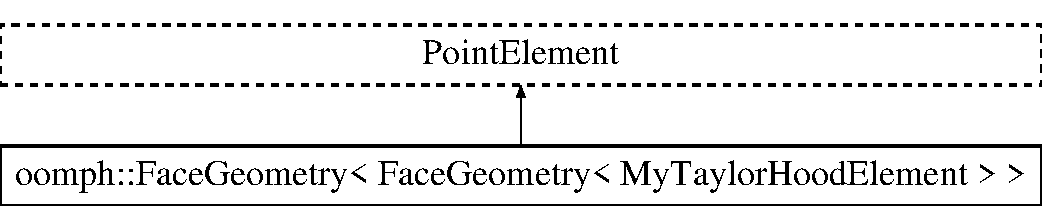
\includegraphics[height=2.000000cm]{classoomph_1_1FaceGeometry_3_01FaceGeometry_3_01MyTaylorHoodElement_01_4_01_4}
\end{center}
\end{figure}
\subsection*{Public Member Functions}
\begin{DoxyCompactItemize}
\item 
\hyperlink{classoomph_1_1FaceGeometry_3_01FaceGeometry_3_01MyTaylorHoodElement_01_4_01_4_a35f1bde1f3b3cc7c29d417cd75f0ef86}{Face\+Geometry} ()
\end{DoxyCompactItemize}


\subsection{Detailed Description}
\subsubsection*{template$<$$>$\newline
class oomph\+::\+Face\+Geometry$<$ Face\+Geometry$<$ My\+Taylor\+Hood\+Element $>$ $>$}

Face geometry for element is the same as that for the underlying wrapped element 

Definition at line 325 of file my\+\_\+taylor\+\_\+hood\+\_\+elements.\+h.



\subsection{Constructor \& Destructor Documentation}
\mbox{\Hypertarget{classoomph_1_1FaceGeometry_3_01FaceGeometry_3_01MyTaylorHoodElement_01_4_01_4_a35f1bde1f3b3cc7c29d417cd75f0ef86}\label{classoomph_1_1FaceGeometry_3_01FaceGeometry_3_01MyTaylorHoodElement_01_4_01_4_a35f1bde1f3b3cc7c29d417cd75f0ef86}} 
\index{oomph\+::\+Face\+Geometry$<$ Face\+Geometry$<$ My\+Taylor\+Hood\+Element $>$ $>$@{oomph\+::\+Face\+Geometry$<$ Face\+Geometry$<$ My\+Taylor\+Hood\+Element $>$ $>$}!Face\+Geometry@{Face\+Geometry}}
\index{Face\+Geometry@{Face\+Geometry}!oomph\+::\+Face\+Geometry$<$ Face\+Geometry$<$ My\+Taylor\+Hood\+Element $>$ $>$@{oomph\+::\+Face\+Geometry$<$ Face\+Geometry$<$ My\+Taylor\+Hood\+Element $>$ $>$}}
\subsubsection{\texorpdfstring{Face\+Geometry()}{FaceGeometry()}}
{\footnotesize\ttfamily oomph\+::\+Face\+Geometry$<$ Face\+Geometry$<$ \hyperlink{classoomph_1_1MyTaylorHoodElement}{My\+Taylor\+Hood\+Element} $>$ $>$\+::Face\+Geometry (\begin{DoxyParamCaption}{ }\end{DoxyParamCaption})\hspace{0.3cm}{\ttfamily [inline]}}



Definition at line 329 of file my\+\_\+taylor\+\_\+hood\+\_\+elements.\+h.



The documentation for this class was generated from the following file\+:\begin{DoxyCompactItemize}
\item 
\hyperlink{my__taylor__hood__elements_8h}{my\+\_\+taylor\+\_\+hood\+\_\+elements.\+h}\end{DoxyCompactItemize}

\hypertarget{classoomph_1_1FaceGeometry_3_01MyTaylorHoodElement_01_4}{}\section{oomph\+:\+:Face\+Geometry$<$ My\+Taylor\+Hood\+Element $>$ Class Template Reference}
\label{classoomph_1_1FaceGeometry_3_01MyTaylorHoodElement_01_4}\index{oomph\+::\+Face\+Geometry$<$ My\+Taylor\+Hood\+Element $>$@{oomph\+::\+Face\+Geometry$<$ My\+Taylor\+Hood\+Element $>$}}


{\ttfamily \#include $<$my\+\_\+taylor\+\_\+hood\+\_\+elements.\+h$>$}

Inheritance diagram for oomph\+:\+:Face\+Geometry$<$ My\+Taylor\+Hood\+Element $>$\+:\begin{figure}[H]
\begin{center}
\leavevmode
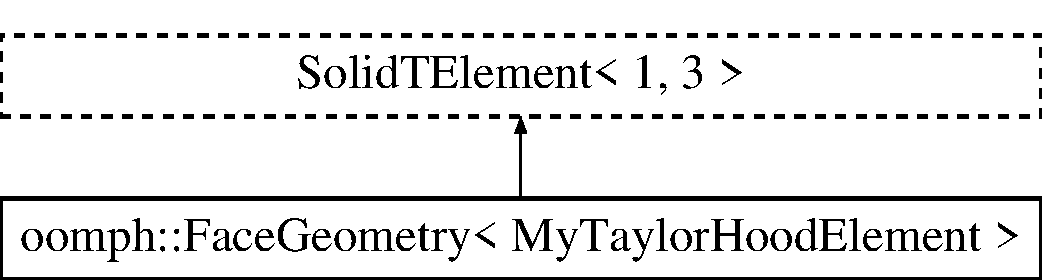
\includegraphics[height=2.000000cm]{classoomph_1_1FaceGeometry_3_01MyTaylorHoodElement_01_4}
\end{center}
\end{figure}
\subsection*{Public Member Functions}
\begin{DoxyCompactItemize}
\item 
\hyperlink{classoomph_1_1FaceGeometry_3_01MyTaylorHoodElement_01_4_a604dfaeec030bb7a08069c0e2c8805ab}{Face\+Geometry} ()
\end{DoxyCompactItemize}


\subsection{Detailed Description}
\subsubsection*{template$<$$>$\newline
class oomph\+::\+Face\+Geometry$<$ My\+Taylor\+Hood\+Element $>$}

Face geometry for element is the same as that for the underlying wrapped element 

Definition at line 313 of file my\+\_\+taylor\+\_\+hood\+\_\+elements.\+h.



\subsection{Constructor \& Destructor Documentation}
\mbox{\Hypertarget{classoomph_1_1FaceGeometry_3_01MyTaylorHoodElement_01_4_a604dfaeec030bb7a08069c0e2c8805ab}\label{classoomph_1_1FaceGeometry_3_01MyTaylorHoodElement_01_4_a604dfaeec030bb7a08069c0e2c8805ab}} 
\index{oomph\+::\+Face\+Geometry$<$ My\+Taylor\+Hood\+Element $>$@{oomph\+::\+Face\+Geometry$<$ My\+Taylor\+Hood\+Element $>$}!Face\+Geometry@{Face\+Geometry}}
\index{Face\+Geometry@{Face\+Geometry}!oomph\+::\+Face\+Geometry$<$ My\+Taylor\+Hood\+Element $>$@{oomph\+::\+Face\+Geometry$<$ My\+Taylor\+Hood\+Element $>$}}
\subsubsection{\texorpdfstring{Face\+Geometry()}{FaceGeometry()}}
{\footnotesize\ttfamily oomph\+::\+Face\+Geometry$<$ \hyperlink{classoomph_1_1MyTaylorHoodElement}{My\+Taylor\+Hood\+Element} $>$\+::Face\+Geometry (\begin{DoxyParamCaption}{ }\end{DoxyParamCaption})\hspace{0.3cm}{\ttfamily [inline]}}



Definition at line 317 of file my\+\_\+taylor\+\_\+hood\+\_\+elements.\+h.



The documentation for this class was generated from the following file\+:\begin{DoxyCompactItemize}
\item 
\hyperlink{my__taylor__hood__elements_8h}{my\+\_\+taylor\+\_\+hood\+\_\+elements.\+h}\end{DoxyCompactItemize}

\hypertarget{classGeneralEllipse}{}\section{General\+Ellipse Class Reference}
\label{classGeneralEllipse}\index{General\+Ellipse@{General\+Ellipse}}


A geometric object for an ellipse with initial centre of mass at (centre\+\_\+x, centre\+\_\+y) with axis in the x direction given by 2a and in the y-\/direction given by 2b. The boundary of the ellipse is parametrised by its angle.  


Inheritance diagram for General\+Ellipse\+:\begin{figure}[H]
\begin{center}
\leavevmode
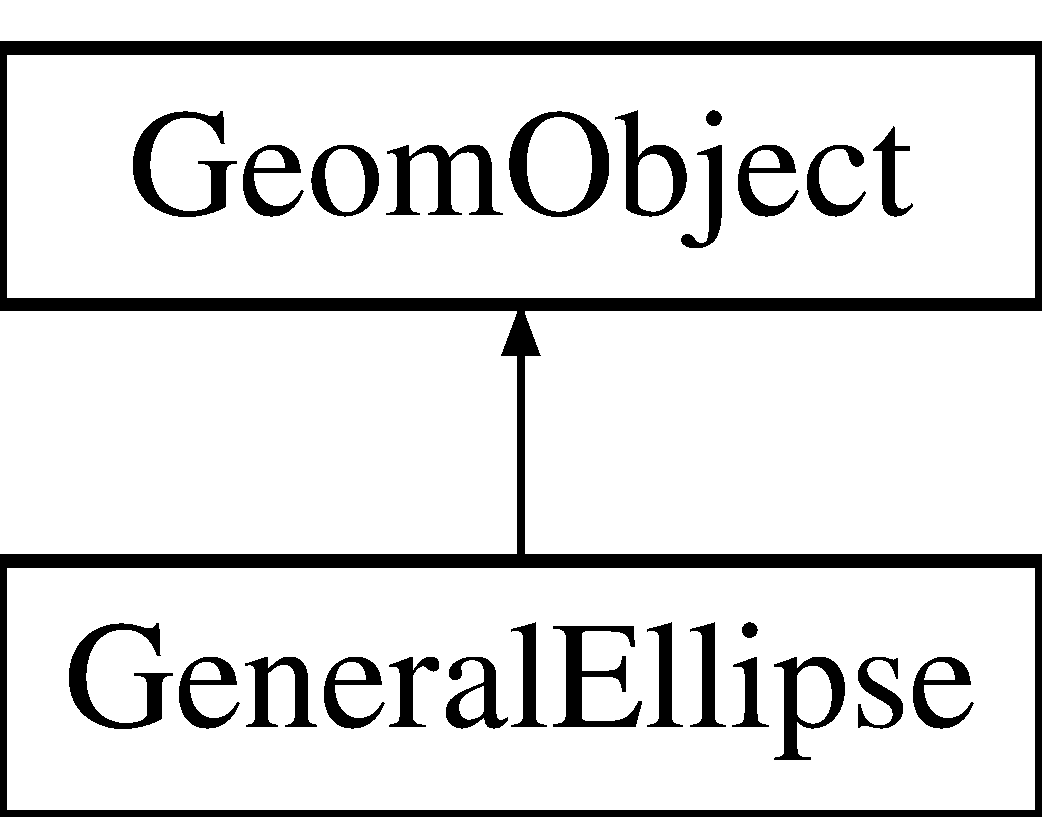
\includegraphics[height=2.000000cm]{classGeneralEllipse}
\end{center}
\end{figure}
\subsection*{Public Member Functions}
\begin{DoxyCompactItemize}
\item 
\hyperlink{classGeneralEllipse_a50dc036d709bcd1d53eafb62b5548f67}{General\+Ellipse} (const double \&centre\+\_\+x, const double \&centre\+\_\+y, const double \&a, const double \&b)
\begin{DoxyCompactList}\small\item\em Simple Constructor that transfers appropriate geometric parameters into internal data. \end{DoxyCompactList}\item 
\hyperlink{classGeneralEllipse_a3ac5c17cf8c4998f1b74913860cb3bb9}{$\sim$\+General\+Ellipse} ()
\begin{DoxyCompactList}\small\item\em Empty Destructor. \end{DoxyCompactList}\item 
void \hyperlink{classGeneralEllipse_a85e975c70441a9c9c711b5e27d124bff}{position} (const Vector$<$ double $>$ \&xi, Vector$<$ double $>$ \&r) const
\item 
void \hyperlink{classGeneralEllipse_a2bdcc69fcb1f1725124d625c032d171a}{position} (const unsigned \&t, const Vector$<$ double $>$ \&xi, Vector$<$ double $>$ \&r) const
\end{DoxyCompactItemize}
\subsection*{Private Attributes}
\begin{DoxyCompactItemize}
\item 
double \hyperlink{classGeneralEllipse_aeb974769f58d136a12ac1532506304cc}{Centre\+\_\+x}
\item 
double \hyperlink{classGeneralEllipse_abf2def5a5140bb35e381b800c4b91dc9}{Centre\+\_\+y}
\item 
double \hyperlink{classGeneralEllipse_ae583e1437da6ad4eb228dda60b61808a}{A}
\item 
double \hyperlink{classGeneralEllipse_a185ae9786d5c6c82eef61e163e9310c6}{B}
\end{DoxyCompactItemize}


\subsection{Detailed Description}
A geometric object for an ellipse with initial centre of mass at (centre\+\_\+x, centre\+\_\+y) with axis in the x direction given by 2a and in the y-\/direction given by 2b. The boundary of the ellipse is parametrised by its angle. 

Definition at line 149 of file jeffery\+\_\+orbit.\+cc.



\subsection{Constructor \& Destructor Documentation}
\mbox{\Hypertarget{classGeneralEllipse_a50dc036d709bcd1d53eafb62b5548f67}\label{classGeneralEllipse_a50dc036d709bcd1d53eafb62b5548f67}} 
\index{General\+Ellipse@{General\+Ellipse}!General\+Ellipse@{General\+Ellipse}}
\index{General\+Ellipse@{General\+Ellipse}!General\+Ellipse@{General\+Ellipse}}
\subsubsection{\texorpdfstring{General\+Ellipse()}{GeneralEllipse()}}
{\footnotesize\ttfamily General\+Ellipse\+::\+General\+Ellipse (\begin{DoxyParamCaption}\item[{const double \&}]{centre\+\_\+x,  }\item[{const double \&}]{centre\+\_\+y,  }\item[{const double \&}]{a,  }\item[{const double \&}]{b }\end{DoxyParamCaption})\hspace{0.3cm}{\ttfamily [inline]}}



Simple Constructor that transfers appropriate geometric parameters into internal data. 



Definition at line 160 of file jeffery\+\_\+orbit.\+cc.

\mbox{\Hypertarget{classGeneralEllipse_a3ac5c17cf8c4998f1b74913860cb3bb9}\label{classGeneralEllipse_a3ac5c17cf8c4998f1b74913860cb3bb9}} 
\index{General\+Ellipse@{General\+Ellipse}!````~General\+Ellipse@{$\sim$\+General\+Ellipse}}
\index{````~General\+Ellipse@{$\sim$\+General\+Ellipse}!General\+Ellipse@{General\+Ellipse}}
\subsubsection{\texorpdfstring{$\sim$\+General\+Ellipse()}{~GeneralEllipse()}}
{\footnotesize\ttfamily General\+Ellipse\+::$\sim$\+General\+Ellipse (\begin{DoxyParamCaption}{ }\end{DoxyParamCaption})\hspace{0.3cm}{\ttfamily [inline]}}



Empty Destructor. 



Definition at line 166 of file jeffery\+\_\+orbit.\+cc.



\subsection{Member Function Documentation}
\mbox{\Hypertarget{classGeneralEllipse_a85e975c70441a9c9c711b5e27d124bff}\label{classGeneralEllipse_a85e975c70441a9c9c711b5e27d124bff}} 
\index{General\+Ellipse@{General\+Ellipse}!position@{position}}
\index{position@{position}!General\+Ellipse@{General\+Ellipse}}
\subsubsection{\texorpdfstring{position()}{position()}\hspace{0.1cm}{\footnotesize\ttfamily [1/2]}}
{\footnotesize\ttfamily void General\+Ellipse\+::position (\begin{DoxyParamCaption}\item[{const Vector$<$ double $>$ \&}]{xi,  }\item[{Vector$<$ double $>$ \&}]{r }\end{DoxyParamCaption}) const\hspace{0.3cm}{\ttfamily [inline]}}

Return the position of the ellipse boundary as a function of the angle xi\mbox{[}0\mbox{]} 

Definition at line 170 of file jeffery\+\_\+orbit.\+cc.

\mbox{\Hypertarget{classGeneralEllipse_a2bdcc69fcb1f1725124d625c032d171a}\label{classGeneralEllipse_a2bdcc69fcb1f1725124d625c032d171a}} 
\index{General\+Ellipse@{General\+Ellipse}!position@{position}}
\index{position@{position}!General\+Ellipse@{General\+Ellipse}}
\subsubsection{\texorpdfstring{position()}{position()}\hspace{0.1cm}{\footnotesize\ttfamily [2/2]}}
{\footnotesize\ttfamily void General\+Ellipse\+::position (\begin{DoxyParamCaption}\item[{const unsigned \&}]{t,  }\item[{const Vector$<$ double $>$ \&}]{xi,  }\item[{Vector$<$ double $>$ \&}]{r }\end{DoxyParamCaption}) const\hspace{0.3cm}{\ttfamily [inline]}}



Definition at line 177 of file jeffery\+\_\+orbit.\+cc.



\subsection{Member Data Documentation}
\mbox{\Hypertarget{classGeneralEllipse_ae583e1437da6ad4eb228dda60b61808a}\label{classGeneralEllipse_ae583e1437da6ad4eb228dda60b61808a}} 
\index{General\+Ellipse@{General\+Ellipse}!A@{A}}
\index{A@{A}!General\+Ellipse@{General\+Ellipse}}
\subsubsection{\texorpdfstring{A}{A}}
{\footnotesize\ttfamily double General\+Ellipse\+::A\hspace{0.3cm}{\ttfamily [private]}}



Definition at line 154 of file jeffery\+\_\+orbit.\+cc.

\mbox{\Hypertarget{classGeneralEllipse_a185ae9786d5c6c82eef61e163e9310c6}\label{classGeneralEllipse_a185ae9786d5c6c82eef61e163e9310c6}} 
\index{General\+Ellipse@{General\+Ellipse}!B@{B}}
\index{B@{B}!General\+Ellipse@{General\+Ellipse}}
\subsubsection{\texorpdfstring{B}{B}}
{\footnotesize\ttfamily double General\+Ellipse\+::B\hspace{0.3cm}{\ttfamily [private]}}



Definition at line 154 of file jeffery\+\_\+orbit.\+cc.

\mbox{\Hypertarget{classGeneralEllipse_aeb974769f58d136a12ac1532506304cc}\label{classGeneralEllipse_aeb974769f58d136a12ac1532506304cc}} 
\index{General\+Ellipse@{General\+Ellipse}!Centre\+\_\+x@{Centre\+\_\+x}}
\index{Centre\+\_\+x@{Centre\+\_\+x}!General\+Ellipse@{General\+Ellipse}}
\subsubsection{\texorpdfstring{Centre\+\_\+x}{Centre\_x}}
{\footnotesize\ttfamily double General\+Ellipse\+::\+Centre\+\_\+x\hspace{0.3cm}{\ttfamily [private]}}



Definition at line 154 of file jeffery\+\_\+orbit.\+cc.

\mbox{\Hypertarget{classGeneralEllipse_abf2def5a5140bb35e381b800c4b91dc9}\label{classGeneralEllipse_abf2def5a5140bb35e381b800c4b91dc9}} 
\index{General\+Ellipse@{General\+Ellipse}!Centre\+\_\+y@{Centre\+\_\+y}}
\index{Centre\+\_\+y@{Centre\+\_\+y}!General\+Ellipse@{General\+Ellipse}}
\subsubsection{\texorpdfstring{Centre\+\_\+y}{Centre\_y}}
{\footnotesize\ttfamily double General\+Ellipse\+::\+Centre\+\_\+y\hspace{0.3cm}{\ttfamily [private]}}



Definition at line 154 of file jeffery\+\_\+orbit.\+cc.



The documentation for this class was generated from the following file\+:\begin{DoxyCompactItemize}
\item 
\hyperlink{jeffery__orbit_8cc}{jeffery\+\_\+orbit.\+cc}\end{DoxyCompactItemize}

\hypertarget{classoomph_1_1MyTaylorHoodElement}{}\section{oomph\+:\+:My\+Taylor\+Hood\+Element Class Reference}
\label{classoomph_1_1MyTaylorHoodElement}\index{oomph\+::\+My\+Taylor\+Hood\+Element@{oomph\+::\+My\+Taylor\+Hood\+Element}}


Overload Taylor\+Hood element to modify output.  




{\ttfamily \#include $<$my\+\_\+taylor\+\_\+hood\+\_\+elements.\+h$>$}

Inheritance diagram for oomph\+:\+:My\+Taylor\+Hood\+Element\+:\begin{figure}[H]
\begin{center}
\leavevmode
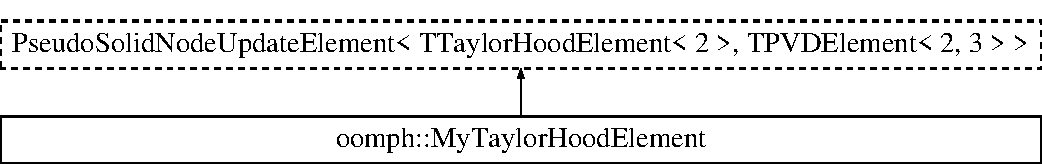
\includegraphics[height=2.000000cm]{classoomph_1_1MyTaylorHoodElement}
\end{center}
\end{figure}
\subsection*{Public Member Functions}
\begin{DoxyCompactItemize}
\item 
\hyperlink{classoomph_1_1MyTaylorHoodElement_a936bd6421ba42e5b73f983f5141b37c2}{My\+Taylor\+Hood\+Element} ()
\begin{DoxyCompactList}\small\item\em Constructor initialise error. \end{DoxyCompactList}\item 
void \hyperlink{classoomph_1_1MyTaylorHoodElement_ae4f6eea59b7bcf6e737d829b37c47fe9}{set\+\_\+error} (const double \&error)
\begin{DoxyCompactList}\small\item\em Set error value for post-\/processing. \end{DoxyCompactList}\item 
std\+::string \hyperlink{classoomph_1_1MyTaylorHoodElement_a429987090e76cd39a657b3a8eefbbbe9}{variable\+\_\+identifier} ()
\begin{DoxyCompactList}\small\item\em Return variable identifier. \end{DoxyCompactList}\item 
void \hyperlink{classoomph_1_1MyTaylorHoodElement_a5505717f2d16c2b231e7c347cb0c49b1}{output} (std\+::ostream \&outfile, const unsigned \&nplot)
\begin{DoxyCompactList}\small\item\em Overload output function. \end{DoxyCompactList}\item 
double \hyperlink{classoomph_1_1MyTaylorHoodElement_ad9efcab0ef22434e6fc5f2eb4b84643d}{square\+\_\+of\+\_\+l2\+\_\+norm} ()
\begin{DoxyCompactList}\small\item\em Get square of L2 norm of velocity. \end{DoxyCompactList}\end{DoxyCompactItemize}
\subsection*{Private Attributes}
\begin{DoxyCompactItemize}
\item 
double \hyperlink{classoomph_1_1MyTaylorHoodElement_a381cf2cdb628fb7aacfd6dd59dc2996b}{Error}
\begin{DoxyCompactList}\small\item\em Storage for elemental error estimate -- used for post-\/processing. \end{DoxyCompactList}\end{DoxyCompactItemize}


\subsection{Detailed Description}
Overload Taylor\+Hood element to modify output. 

Definition at line 39 of file my\+\_\+taylor\+\_\+hood\+\_\+elements.\+h.



\subsection{Constructor \& Destructor Documentation}
\mbox{\Hypertarget{classoomph_1_1MyTaylorHoodElement_a936bd6421ba42e5b73f983f5141b37c2}\label{classoomph_1_1MyTaylorHoodElement_a936bd6421ba42e5b73f983f5141b37c2}} 
\index{oomph\+::\+My\+Taylor\+Hood\+Element@{oomph\+::\+My\+Taylor\+Hood\+Element}!My\+Taylor\+Hood\+Element@{My\+Taylor\+Hood\+Element}}
\index{My\+Taylor\+Hood\+Element@{My\+Taylor\+Hood\+Element}!oomph\+::\+My\+Taylor\+Hood\+Element@{oomph\+::\+My\+Taylor\+Hood\+Element}}
\subsubsection{\texorpdfstring{My\+Taylor\+Hood\+Element()}{MyTaylorHoodElement()}}
{\footnotesize\ttfamily oomph\+::\+My\+Taylor\+Hood\+Element\+::\+My\+Taylor\+Hood\+Element (\begin{DoxyParamCaption}{ }\end{DoxyParamCaption})\hspace{0.3cm}{\ttfamily [inline]}}



Constructor initialise error. 



Definition at line 52 of file my\+\_\+taylor\+\_\+hood\+\_\+elements.\+h.



\subsection{Member Function Documentation}
\mbox{\Hypertarget{classoomph_1_1MyTaylorHoodElement_a5505717f2d16c2b231e7c347cb0c49b1}\label{classoomph_1_1MyTaylorHoodElement_a5505717f2d16c2b231e7c347cb0c49b1}} 
\index{oomph\+::\+My\+Taylor\+Hood\+Element@{oomph\+::\+My\+Taylor\+Hood\+Element}!output@{output}}
\index{output@{output}!oomph\+::\+My\+Taylor\+Hood\+Element@{oomph\+::\+My\+Taylor\+Hood\+Element}}
\subsubsection{\texorpdfstring{output()}{output()}}
{\footnotesize\ttfamily void oomph\+::\+My\+Taylor\+Hood\+Element\+::output (\begin{DoxyParamCaption}\item[{std\+::ostream \&}]{outfile,  }\item[{const unsigned \&}]{nplot }\end{DoxyParamCaption})\hspace{0.3cm}{\ttfamily [inline]}}



Overload output function. 



Definition at line 89 of file my\+\_\+taylor\+\_\+hood\+\_\+elements.\+h.

\mbox{\Hypertarget{classoomph_1_1MyTaylorHoodElement_ae4f6eea59b7bcf6e737d829b37c47fe9}\label{classoomph_1_1MyTaylorHoodElement_ae4f6eea59b7bcf6e737d829b37c47fe9}} 
\index{oomph\+::\+My\+Taylor\+Hood\+Element@{oomph\+::\+My\+Taylor\+Hood\+Element}!set\+\_\+error@{set\+\_\+error}}
\index{set\+\_\+error@{set\+\_\+error}!oomph\+::\+My\+Taylor\+Hood\+Element@{oomph\+::\+My\+Taylor\+Hood\+Element}}
\subsubsection{\texorpdfstring{set\+\_\+error()}{set\_error()}}
{\footnotesize\ttfamily void oomph\+::\+My\+Taylor\+Hood\+Element\+::set\+\_\+error (\begin{DoxyParamCaption}\item[{const double \&}]{error }\end{DoxyParamCaption})\hspace{0.3cm}{\ttfamily [inline]}}



Set error value for post-\/processing. 



Definition at line 58 of file my\+\_\+taylor\+\_\+hood\+\_\+elements.\+h.

\mbox{\Hypertarget{classoomph_1_1MyTaylorHoodElement_ad9efcab0ef22434e6fc5f2eb4b84643d}\label{classoomph_1_1MyTaylorHoodElement_ad9efcab0ef22434e6fc5f2eb4b84643d}} 
\index{oomph\+::\+My\+Taylor\+Hood\+Element@{oomph\+::\+My\+Taylor\+Hood\+Element}!square\+\_\+of\+\_\+l2\+\_\+norm@{square\+\_\+of\+\_\+l2\+\_\+norm}}
\index{square\+\_\+of\+\_\+l2\+\_\+norm@{square\+\_\+of\+\_\+l2\+\_\+norm}!oomph\+::\+My\+Taylor\+Hood\+Element@{oomph\+::\+My\+Taylor\+Hood\+Element}}
\subsubsection{\texorpdfstring{square\+\_\+of\+\_\+l2\+\_\+norm()}{square\_of\_l2\_norm()}}
{\footnotesize\ttfamily double oomph\+::\+My\+Taylor\+Hood\+Element\+::square\+\_\+of\+\_\+l2\+\_\+norm (\begin{DoxyParamCaption}{ }\end{DoxyParamCaption})\hspace{0.3cm}{\ttfamily [inline]}}



Get square of L2 norm of velocity. 



Definition at line 235 of file my\+\_\+taylor\+\_\+hood\+\_\+elements.\+h.

\mbox{\Hypertarget{classoomph_1_1MyTaylorHoodElement_a429987090e76cd39a657b3a8eefbbbe9}\label{classoomph_1_1MyTaylorHoodElement_a429987090e76cd39a657b3a8eefbbbe9}} 
\index{oomph\+::\+My\+Taylor\+Hood\+Element@{oomph\+::\+My\+Taylor\+Hood\+Element}!variable\+\_\+identifier@{variable\+\_\+identifier}}
\index{variable\+\_\+identifier@{variable\+\_\+identifier}!oomph\+::\+My\+Taylor\+Hood\+Element@{oomph\+::\+My\+Taylor\+Hood\+Element}}
\subsubsection{\texorpdfstring{variable\+\_\+identifier()}{variable\_identifier()}}
{\footnotesize\ttfamily std\+::string oomph\+::\+My\+Taylor\+Hood\+Element\+::variable\+\_\+identifier (\begin{DoxyParamCaption}{ }\end{DoxyParamCaption})\hspace{0.3cm}{\ttfamily [inline]}}



Return variable identifier. 



Definition at line 61 of file my\+\_\+taylor\+\_\+hood\+\_\+elements.\+h.



\subsection{Member Data Documentation}
\mbox{\Hypertarget{classoomph_1_1MyTaylorHoodElement_a381cf2cdb628fb7aacfd6dd59dc2996b}\label{classoomph_1_1MyTaylorHoodElement_a381cf2cdb628fb7aacfd6dd59dc2996b}} 
\index{oomph\+::\+My\+Taylor\+Hood\+Element@{oomph\+::\+My\+Taylor\+Hood\+Element}!Error@{Error}}
\index{Error@{Error}!oomph\+::\+My\+Taylor\+Hood\+Element@{oomph\+::\+My\+Taylor\+Hood\+Element}}
\subsubsection{\texorpdfstring{Error}{Error}}
{\footnotesize\ttfamily double oomph\+::\+My\+Taylor\+Hood\+Element\+::\+Error\hspace{0.3cm}{\ttfamily [private]}}



Storage for elemental error estimate -- used for post-\/processing. 



Definition at line 47 of file my\+\_\+taylor\+\_\+hood\+\_\+elements.\+h.



The documentation for this class was generated from the following file\+:\begin{DoxyCompactItemize}
\item 
\hyperlink{my__taylor__hood__elements_8h}{my\+\_\+taylor\+\_\+hood\+\_\+elements.\+h}\end{DoxyCompactItemize}

\hypertarget{classUnstructuredImmersedEllipseProblem}{}\section{Unstructured\+Immersed\+Ellipse\+Problem$<$ E\+L\+E\+M\+E\+NT $>$ Class Template Reference}
\label{classUnstructuredImmersedEllipseProblem}\index{Unstructured\+Immersed\+Ellipse\+Problem$<$ E\+L\+E\+M\+E\+N\+T $>$@{Unstructured\+Immersed\+Ellipse\+Problem$<$ E\+L\+E\+M\+E\+N\+T $>$}}
Inheritance diagram for Unstructured\+Immersed\+Ellipse\+Problem$<$ E\+L\+E\+M\+E\+NT $>$\+:\begin{figure}[H]
\begin{center}
\leavevmode
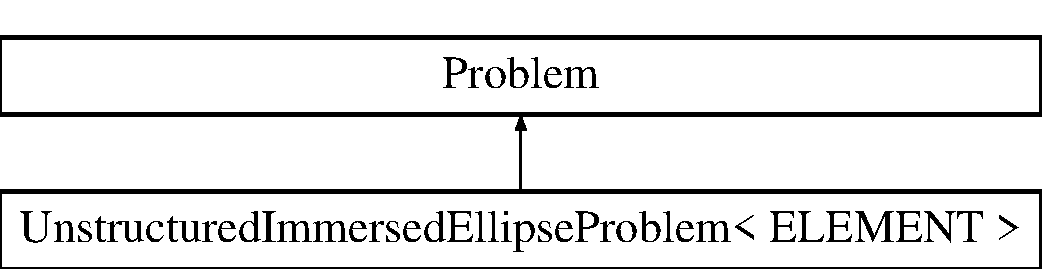
\includegraphics[height=2.000000cm]{classUnstructuredImmersedEllipseProblem}
\end{center}
\end{figure}
\subsection*{Public Member Functions}
\begin{DoxyCompactItemize}
\item 
\hyperlink{classUnstructuredImmersedEllipseProblem_a544a35f261200bb4a4e29a88faa1a69c}{Unstructured\+Immersed\+Ellipse\+Problem} ()
\begin{DoxyCompactList}\small\item\em Constructor. \end{DoxyCompactList}\item 
\hyperlink{classUnstructuredImmersedEllipseProblem_a84cdf81be59fc646eb4d5b3bc0ff4280}{$\sim$\+Unstructured\+Immersed\+Ellipse\+Problem} ()
\begin{DoxyCompactList}\small\item\em Destructor. \end{DoxyCompactList}\item 
void \hyperlink{classUnstructuredImmersedEllipseProblem_a368c412c4c9a9e9403b4e67d3582e3a5}{actions\+\_\+before\+\_\+implicit\+\_\+timestep} ()
\begin{DoxyCompactList}\small\item\em Reset the boundary conditions when timestepping. \end{DoxyCompactList}\item 
void \hyperlink{classUnstructuredImmersedEllipseProblem_aa560217a33a9a9bc150fbdf15dbf1877}{actions\+\_\+before\+\_\+adapt} ()
\begin{DoxyCompactList}\small\item\em Wipe the meshes of Lagrange multiplier and drag elements. \end{DoxyCompactList}\item 
void \hyperlink{classUnstructuredImmersedEllipseProblem_ab1558b409285aea617f4abf7d3a64b3d}{actions\+\_\+after\+\_\+adapt} ()
\begin{DoxyCompactList}\small\item\em Rebuild the meshes of Lagrange multiplier and drag elements. \end{DoxyCompactList}\item 
void \hyperlink{classUnstructuredImmersedEllipseProblem_afa51876a2af9dd7640ff1f5a434804bf}{actions\+\_\+before\+\_\+newton\+\_\+convergence\+\_\+check} ()
\begin{DoxyCompactList}\small\item\em Re-\/apply the no slip condition (imposed indirectly via enslaved velocities) \end{DoxyCompactList}\item 
void \hyperlink{classUnstructuredImmersedEllipseProblem_a42b13e3306ff2a94053907644ba17c8d}{complete\+\_\+problem\+\_\+setup} ()
\begin{DoxyCompactList}\small\item\em Set boundary condition, assign auxiliary node update fct. Complete the build of all elements, attach power elements that allow computation of drag vector. \end{DoxyCompactList}\item 
void \hyperlink{classUnstructuredImmersedEllipseProblem_ab201b187b240105fd8d444d943f6dada}{set\+\_\+boundary\+\_\+velocity} ()
\begin{DoxyCompactList}\small\item\em Set the boundary velocity. \end{DoxyCompactList}\item 
void \hyperlink{classUnstructuredImmersedEllipseProblem_a2a88b40ff1988de0fc696f1eb755ea54}{solve\+\_\+for\+\_\+consistent\+\_\+nodal\+\_\+positions} ()
\begin{DoxyCompactList}\small\item\em Function that solves a simplified problem to ensure that the positions of the boundary nodes are initially consistent with the lagrange multiplier formulation. \end{DoxyCompactList}\item 
void \hyperlink{classUnstructuredImmersedEllipseProblem_a08e12dd83c98f96e14e8152cc758d398}{doc\+\_\+solution} (const bool \&project=false)
\begin{DoxyCompactList}\small\item\em Doc the solution. \end{DoxyCompactList}\item 
void \hyperlink{classUnstructuredImmersedEllipseProblem_a29a232dfac18ea901332bebdc14fad15}{output\+\_\+exact\+\_\+solution} (std\+::ofstream \&output\+\_\+file)
\begin{DoxyCompactList}\small\item\em Output the exact solution. \end{DoxyCompactList}\end{DoxyCompactItemize}
\subsection*{Private Member Functions}
\begin{DoxyCompactItemize}
\item 
void \hyperlink{classUnstructuredImmersedEllipseProblem_a3b4a4e279a11b37d79d040b348008765}{create\+\_\+lagrange\+\_\+multiplier\+\_\+elements} ()
\begin{DoxyCompactList}\small\item\em Create elements that enforce prescribed boundary motion for the pseudo-\/solid fluid mesh by Lagrange multipliers. \end{DoxyCompactList}\item 
void \hyperlink{classUnstructuredImmersedEllipseProblem_a51555f77dc360c94591ee68c3fc9928a}{delete\+\_\+lagrange\+\_\+multiplier\+\_\+elements} ()
\begin{DoxyCompactList}\small\item\em Delete elements that impose the prescribed boundary displacement and wipe the associated mesh. \end{DoxyCompactList}\item 
void \hyperlink{classUnstructuredImmersedEllipseProblem_a16a7c6022867f709ebdd59b8fee2004a}{create\+\_\+drag\+\_\+elements} ()
\begin{DoxyCompactList}\small\item\em Create elements that calculate the drag and torque on the boundaries. \end{DoxyCompactList}\item 
void \hyperlink{classUnstructuredImmersedEllipseProblem_a7d7b84968988d37091b29957b0af5bfa}{delete\+\_\+drag\+\_\+elements} ()
\begin{DoxyCompactList}\small\item\em Delete elements that calculate the drag and torque on the boundaries. \end{DoxyCompactList}\item 
void \hyperlink{classUnstructuredImmersedEllipseProblem_a07dc16909c0223fe4b656fd270f27c11}{pin\+\_\+rigid\+\_\+body} ()
\begin{DoxyCompactList}\small\item\em Pin the degrees of freedom associated with the solid bodies. \end{DoxyCompactList}\item 
void \hyperlink{classUnstructuredImmersedEllipseProblem_a4f8c7e7e4d626084f6515a152b165567}{unpin\+\_\+rigid\+\_\+body} ()
\begin{DoxyCompactList}\small\item\em Unpin the degrees of freedom associated with the solid bodies. \end{DoxyCompactList}\end{DoxyCompactItemize}
\subsection*{Private Attributes}
\begin{DoxyCompactItemize}
\item 
Solid\+Mesh $\ast$ \hyperlink{classUnstructuredImmersedEllipseProblem_ad644e67ccd6ab0811c5fe2b7b944fbca}{Lagrange\+\_\+multiplier\+\_\+mesh\+\_\+pt}
\begin{DoxyCompactList}\small\item\em Pointers to mesh of Lagrange multiplier elements. \end{DoxyCompactList}\item 
Refineable\+Solid\+Triangle\+Mesh$<$ E\+L\+E\+M\+E\+NT $>$ $\ast$ \hyperlink{classUnstructuredImmersedEllipseProblem_a0ba79ccde26b781b66d9839460f08bd3}{Fluid\+\_\+mesh\+\_\+pt}
\begin{DoxyCompactList}\small\item\em Pointer to Fluid\+\_\+mesh. \end{DoxyCompactList}\item 
Triangle\+Mesh\+Polygon $\ast$ \hyperlink{classUnstructuredImmersedEllipseProblem_ae0b35188432c371804887b6de86b48c7}{Outer\+\_\+boundary\+\_\+polygon\+\_\+pt}
\begin{DoxyCompactList}\small\item\em Triangle mesh polygon for outer boundary. \end{DoxyCompactList}\item 
Vector$<$ Mesh $\ast$ $>$ \hyperlink{classUnstructuredImmersedEllipseProblem_a9b4d04277b1f42c9428b610968f6f10d}{Drag\+\_\+mesh\+\_\+pt}
\begin{DoxyCompactList}\small\item\em Mesh of drag elements. \end{DoxyCompactList}\item 
Mesh $\ast$ \hyperlink{classUnstructuredImmersedEllipseProblem_a34f1376227d4b995678eedd77813388b}{Rigid\+\_\+body\+\_\+mesh\+\_\+pt}
\begin{DoxyCompactList}\small\item\em Mesh of the generalised elements for the rigid bodies. \end{DoxyCompactList}\item 
Vector$<$ Geom\+Object $\ast$ $>$ \hyperlink{classUnstructuredImmersedEllipseProblem_aaa6d1c19f3634a6f08f3dd7e5046217e}{Rigid\+\_\+body\+\_\+pt}
\begin{DoxyCompactList}\small\item\em Storage for the geom object. \end{DoxyCompactList}\item 
Doc\+Info \hyperlink{classUnstructuredImmersedEllipseProblem_a1c463ed904f01e6466baae0533c79780}{Doc\+\_\+info}
\begin{DoxyCompactList}\small\item\em Internal Doc\+Info object. \end{DoxyCompactList}\item 
ofstream \hyperlink{classUnstructuredImmersedEllipseProblem_a71a3b24b610e05f7be916c4214dab8dc}{Norm\+\_\+file}
\begin{DoxyCompactList}\small\item\em File to document the norm of the solution (for validation purposes) \end{DoxyCompactList}\item 
ofstream \hyperlink{classUnstructuredImmersedEllipseProblem_acd1e8ec8e510f029f449f13dfdebbc99}{Cog\+\_\+file}
\begin{DoxyCompactList}\small\item\em File to document the motion of the centre of gravity. \end{DoxyCompactList}\item 
ofstream \hyperlink{classUnstructuredImmersedEllipseProblem_a3dc1ec2e066466a6f228864b873d95fa}{Cog\+\_\+exact\+\_\+file}
\begin{DoxyCompactList}\small\item\em File to document the exact motion of the centre of gravity. \end{DoxyCompactList}\end{DoxyCompactItemize}


\subsection{Detailed Description}
\subsubsection*{template$<$class E\+L\+E\+M\+E\+NT$>$\newline
class Unstructured\+Immersed\+Ellipse\+Problem$<$ E\+L\+E\+M\+E\+N\+T $>$}

Unstructured Navier-\/\+Stokes A\+LE Problem for a rigid ellipse immersed within a viscous fluid 

Definition at line 197 of file jeffery\+\_\+orbit.\+cc.



\subsection{Constructor \& Destructor Documentation}
\mbox{\Hypertarget{classUnstructuredImmersedEllipseProblem_a544a35f261200bb4a4e29a88faa1a69c}\label{classUnstructuredImmersedEllipseProblem_a544a35f261200bb4a4e29a88faa1a69c}} 
\index{Unstructured\+Immersed\+Ellipse\+Problem@{Unstructured\+Immersed\+Ellipse\+Problem}!Unstructured\+Immersed\+Ellipse\+Problem@{Unstructured\+Immersed\+Ellipse\+Problem}}
\index{Unstructured\+Immersed\+Ellipse\+Problem@{Unstructured\+Immersed\+Ellipse\+Problem}!Unstructured\+Immersed\+Ellipse\+Problem@{Unstructured\+Immersed\+Ellipse\+Problem}}
\subsubsection{\texorpdfstring{Unstructured\+Immersed\+Ellipse\+Problem()}{UnstructuredImmersedEllipseProblem()}}
{\footnotesize\ttfamily template$<$class E\+L\+E\+M\+E\+NT $>$ \\
\hyperlink{classUnstructuredImmersedEllipseProblem}{Unstructured\+Immersed\+Ellipse\+Problem}$<$ E\+L\+E\+M\+E\+NT $>$\+::\hyperlink{classUnstructuredImmersedEllipseProblem}{Unstructured\+Immersed\+Ellipse\+Problem} (\begin{DoxyParamCaption}{ }\end{DoxyParamCaption})}



Constructor. 

Constructor\+: Open output files, construct time steppers, build fluid mesh, immersed rigid body and combine to form the problem 

Definition at line 310 of file jeffery\+\_\+orbit.\+cc.



References Problem\+\_\+\+Parameter\+::A, Problem\+\_\+\+Parameter\+::B, Problem\+\_\+\+Parameter\+::\+Density\+\_\+ratio, Problem\+\_\+\+Parameter\+::\+Re, Problem\+\_\+\+Parameter\+::\+St, and Unstructured\+Immersed\+Ellipse\+Problem$<$ E\+L\+E\+M\+E\+N\+T $>$\+::$\sim$\+Unstructured\+Immersed\+Ellipse\+Problem().

\mbox{\Hypertarget{classUnstructuredImmersedEllipseProblem_a84cdf81be59fc646eb4d5b3bc0ff4280}\label{classUnstructuredImmersedEllipseProblem_a84cdf81be59fc646eb4d5b3bc0ff4280}} 
\index{Unstructured\+Immersed\+Ellipse\+Problem@{Unstructured\+Immersed\+Ellipse\+Problem}!````~Unstructured\+Immersed\+Ellipse\+Problem@{$\sim$\+Unstructured\+Immersed\+Ellipse\+Problem}}
\index{````~Unstructured\+Immersed\+Ellipse\+Problem@{$\sim$\+Unstructured\+Immersed\+Ellipse\+Problem}!Unstructured\+Immersed\+Ellipse\+Problem@{Unstructured\+Immersed\+Ellipse\+Problem}}
\subsubsection{\texorpdfstring{$\sim$\+Unstructured\+Immersed\+Ellipse\+Problem()}{~UnstructuredImmersedEllipseProblem()}}
{\footnotesize\ttfamily template$<$class E\+L\+E\+M\+E\+NT $>$ \\
\hyperlink{classUnstructuredImmersedEllipseProblem}{Unstructured\+Immersed\+Ellipse\+Problem}$<$ E\+L\+E\+M\+E\+NT $>$\+::$\sim$\hyperlink{classUnstructuredImmersedEllipseProblem}{Unstructured\+Immersed\+Ellipse\+Problem} (\begin{DoxyParamCaption}{ }\end{DoxyParamCaption})}



Destructor. 

Destructor that cleans up memory and closes files. 

Definition at line 557 of file jeffery\+\_\+orbit.\+cc.



References Problem\+\_\+\+Parameter\+::\+Constitutive\+\_\+law\+\_\+pt.



Referenced by Unstructured\+Immersed\+Ellipse\+Problem$<$ E\+L\+E\+M\+E\+N\+T $>$\+::\+Unstructured\+Immersed\+Ellipse\+Problem().



\subsection{Member Function Documentation}
\mbox{\Hypertarget{classUnstructuredImmersedEllipseProblem_ab1558b409285aea617f4abf7d3a64b3d}\label{classUnstructuredImmersedEllipseProblem_ab1558b409285aea617f4abf7d3a64b3d}} 
\index{Unstructured\+Immersed\+Ellipse\+Problem@{Unstructured\+Immersed\+Ellipse\+Problem}!actions\+\_\+after\+\_\+adapt@{actions\+\_\+after\+\_\+adapt}}
\index{actions\+\_\+after\+\_\+adapt@{actions\+\_\+after\+\_\+adapt}!Unstructured\+Immersed\+Ellipse\+Problem@{Unstructured\+Immersed\+Ellipse\+Problem}}
\subsubsection{\texorpdfstring{actions\+\_\+after\+\_\+adapt()}{actions\_after\_adapt()}}
{\footnotesize\ttfamily template$<$class E\+L\+E\+M\+E\+NT $>$ \\
void \hyperlink{classUnstructuredImmersedEllipseProblem}{Unstructured\+Immersed\+Ellipse\+Problem}$<$ E\+L\+E\+M\+E\+NT $>$\+::actions\+\_\+after\+\_\+adapt (\begin{DoxyParamCaption}{ }\end{DoxyParamCaption})}



Rebuild the meshes of Lagrange multiplier and drag elements. 

Actions after adapt\+: Rebuild the mesh of Lagrange multiplier elements. 

Definition at line 622 of file jeffery\+\_\+orbit.\+cc.

\mbox{\Hypertarget{classUnstructuredImmersedEllipseProblem_aa560217a33a9a9bc150fbdf15dbf1877}\label{classUnstructuredImmersedEllipseProblem_aa560217a33a9a9bc150fbdf15dbf1877}} 
\index{Unstructured\+Immersed\+Ellipse\+Problem@{Unstructured\+Immersed\+Ellipse\+Problem}!actions\+\_\+before\+\_\+adapt@{actions\+\_\+before\+\_\+adapt}}
\index{actions\+\_\+before\+\_\+adapt@{actions\+\_\+before\+\_\+adapt}!Unstructured\+Immersed\+Ellipse\+Problem@{Unstructured\+Immersed\+Ellipse\+Problem}}
\subsubsection{\texorpdfstring{actions\+\_\+before\+\_\+adapt()}{actions\_before\_adapt()}}
{\footnotesize\ttfamily template$<$class E\+L\+E\+M\+E\+NT $>$ \\
void \hyperlink{classUnstructuredImmersedEllipseProblem}{Unstructured\+Immersed\+Ellipse\+Problem}$<$ E\+L\+E\+M\+E\+NT $>$\+::actions\+\_\+before\+\_\+adapt (\begin{DoxyParamCaption}{ }\end{DoxyParamCaption})}



Wipe the meshes of Lagrange multiplier and drag elements. 

Actions before adapt\+: Wipe the mesh of Lagrange multiplier elements. 

Definition at line 601 of file jeffery\+\_\+orbit.\+cc.

\mbox{\Hypertarget{classUnstructuredImmersedEllipseProblem_a368c412c4c9a9e9403b4e67d3582e3a5}\label{classUnstructuredImmersedEllipseProblem_a368c412c4c9a9e9403b4e67d3582e3a5}} 
\index{Unstructured\+Immersed\+Ellipse\+Problem@{Unstructured\+Immersed\+Ellipse\+Problem}!actions\+\_\+before\+\_\+implicit\+\_\+timestep@{actions\+\_\+before\+\_\+implicit\+\_\+timestep}}
\index{actions\+\_\+before\+\_\+implicit\+\_\+timestep@{actions\+\_\+before\+\_\+implicit\+\_\+timestep}!Unstructured\+Immersed\+Ellipse\+Problem@{Unstructured\+Immersed\+Ellipse\+Problem}}
\subsubsection{\texorpdfstring{actions\+\_\+before\+\_\+implicit\+\_\+timestep()}{actions\_before\_implicit\_timestep()}}
{\footnotesize\ttfamily template$<$class E\+L\+E\+M\+E\+NT $>$ \\
void \hyperlink{classUnstructuredImmersedEllipseProblem}{Unstructured\+Immersed\+Ellipse\+Problem}$<$ E\+L\+E\+M\+E\+NT $>$\+::actions\+\_\+before\+\_\+implicit\+\_\+timestep (\begin{DoxyParamCaption}{ }\end{DoxyParamCaption})\hspace{0.3cm}{\ttfamily [inline]}}



Reset the boundary conditions when timestepping. 



Definition at line 209 of file jeffery\+\_\+orbit.\+cc.

\mbox{\Hypertarget{classUnstructuredImmersedEllipseProblem_afa51876a2af9dd7640ff1f5a434804bf}\label{classUnstructuredImmersedEllipseProblem_afa51876a2af9dd7640ff1f5a434804bf}} 
\index{Unstructured\+Immersed\+Ellipse\+Problem@{Unstructured\+Immersed\+Ellipse\+Problem}!actions\+\_\+before\+\_\+newton\+\_\+convergence\+\_\+check@{actions\+\_\+before\+\_\+newton\+\_\+convergence\+\_\+check}}
\index{actions\+\_\+before\+\_\+newton\+\_\+convergence\+\_\+check@{actions\+\_\+before\+\_\+newton\+\_\+convergence\+\_\+check}!Unstructured\+Immersed\+Ellipse\+Problem@{Unstructured\+Immersed\+Ellipse\+Problem}}
\subsubsection{\texorpdfstring{actions\+\_\+before\+\_\+newton\+\_\+convergence\+\_\+check()}{actions\_before\_newton\_convergence\_check()}}
{\footnotesize\ttfamily template$<$class E\+L\+E\+M\+E\+NT $>$ \\
void \hyperlink{classUnstructuredImmersedEllipseProblem}{Unstructured\+Immersed\+Ellipse\+Problem}$<$ E\+L\+E\+M\+E\+NT $>$\+::actions\+\_\+before\+\_\+newton\+\_\+convergence\+\_\+check (\begin{DoxyParamCaption}{ }\end{DoxyParamCaption})\hspace{0.3cm}{\ttfamily [inline]}}



Re-\/apply the no slip condition (imposed indirectly via enslaved velocities) 



Definition at line 222 of file jeffery\+\_\+orbit.\+cc.

\mbox{\Hypertarget{classUnstructuredImmersedEllipseProblem_a42b13e3306ff2a94053907644ba17c8d}\label{classUnstructuredImmersedEllipseProblem_a42b13e3306ff2a94053907644ba17c8d}} 
\index{Unstructured\+Immersed\+Ellipse\+Problem@{Unstructured\+Immersed\+Ellipse\+Problem}!complete\+\_\+problem\+\_\+setup@{complete\+\_\+problem\+\_\+setup}}
\index{complete\+\_\+problem\+\_\+setup@{complete\+\_\+problem\+\_\+setup}!Unstructured\+Immersed\+Ellipse\+Problem@{Unstructured\+Immersed\+Ellipse\+Problem}}
\subsubsection{\texorpdfstring{complete\+\_\+problem\+\_\+setup()}{complete\_problem\_setup()}}
{\footnotesize\ttfamily template$<$class E\+L\+E\+M\+E\+NT $>$ \\
void \hyperlink{classUnstructuredImmersedEllipseProblem}{Unstructured\+Immersed\+Ellipse\+Problem}$<$ E\+L\+E\+M\+E\+NT $>$\+::complete\+\_\+problem\+\_\+setup (\begin{DoxyParamCaption}{ }\end{DoxyParamCaption})}



Set boundary condition, assign auxiliary node update fct. Complete the build of all elements, attach power elements that allow computation of drag vector. 



Definition at line 658 of file jeffery\+\_\+orbit.\+cc.



References Problem\+\_\+\+Parameter\+::\+Constitutive\+\_\+law\+\_\+pt, Problem\+\_\+\+Parameter\+::\+Lambda\+\_\+sq, Problem\+\_\+\+Parameter\+::\+Re, and Unstructured\+Immersed\+Ellipse\+Problem$<$ E\+L\+E\+M\+E\+N\+T $>$\+::set\+\_\+boundary\+\_\+velocity().

\mbox{\Hypertarget{classUnstructuredImmersedEllipseProblem_a16a7c6022867f709ebdd59b8fee2004a}\label{classUnstructuredImmersedEllipseProblem_a16a7c6022867f709ebdd59b8fee2004a}} 
\index{Unstructured\+Immersed\+Ellipse\+Problem@{Unstructured\+Immersed\+Ellipse\+Problem}!create\+\_\+drag\+\_\+elements@{create\+\_\+drag\+\_\+elements}}
\index{create\+\_\+drag\+\_\+elements@{create\+\_\+drag\+\_\+elements}!Unstructured\+Immersed\+Ellipse\+Problem@{Unstructured\+Immersed\+Ellipse\+Problem}}
\subsubsection{\texorpdfstring{create\+\_\+drag\+\_\+elements()}{create\_drag\_elements()}}
{\footnotesize\ttfamily template$<$class E\+L\+E\+M\+E\+NT $>$ \\
void \hyperlink{classUnstructuredImmersedEllipseProblem}{Unstructured\+Immersed\+Ellipse\+Problem}$<$ E\+L\+E\+M\+E\+NT $>$\+::create\+\_\+drag\+\_\+elements (\begin{DoxyParamCaption}{ }\end{DoxyParamCaption})\hspace{0.3cm}{\ttfamily [private]}}



Create elements that calculate the drag and torque on the boundaries. 

Create elements that calculate the drag and torque on the obstacles in the fluid mesh 

Definition at line 1010 of file jeffery\+\_\+orbit.\+cc.

\mbox{\Hypertarget{classUnstructuredImmersedEllipseProblem_a3b4a4e279a11b37d79d040b348008765}\label{classUnstructuredImmersedEllipseProblem_a3b4a4e279a11b37d79d040b348008765}} 
\index{Unstructured\+Immersed\+Ellipse\+Problem@{Unstructured\+Immersed\+Ellipse\+Problem}!create\+\_\+lagrange\+\_\+multiplier\+\_\+elements@{create\+\_\+lagrange\+\_\+multiplier\+\_\+elements}}
\index{create\+\_\+lagrange\+\_\+multiplier\+\_\+elements@{create\+\_\+lagrange\+\_\+multiplier\+\_\+elements}!Unstructured\+Immersed\+Ellipse\+Problem@{Unstructured\+Immersed\+Ellipse\+Problem}}
\subsubsection{\texorpdfstring{create\+\_\+lagrange\+\_\+multiplier\+\_\+elements()}{create\_lagrange\_multiplier\_elements()}}
{\footnotesize\ttfamily template$<$class E\+L\+E\+M\+E\+NT $>$ \\
void \hyperlink{classUnstructuredImmersedEllipseProblem}{Unstructured\+Immersed\+Ellipse\+Problem}$<$ E\+L\+E\+M\+E\+NT $>$\+::create\+\_\+lagrange\+\_\+multiplier\+\_\+elements (\begin{DoxyParamCaption}{ }\end{DoxyParamCaption})\hspace{0.3cm}{\ttfamily [private]}}



Create elements that enforce prescribed boundary motion for the pseudo-\/solid fluid mesh by Lagrange multipliers. 

Create elements that impose the prescribed boundary displacement for the pseudo-\/solid fluid mesh 

Definition at line 902 of file jeffery\+\_\+orbit.\+cc.



References Unstructured\+Immersed\+Ellipse\+Problem$<$ E\+L\+E\+M\+E\+N\+T $>$\+::delete\+\_\+lagrange\+\_\+multiplier\+\_\+elements().



Referenced by Unstructured\+Immersed\+Ellipse\+Problem$<$ E\+L\+E\+M\+E\+N\+T $>$\+::solve\+\_\+for\+\_\+consistent\+\_\+nodal\+\_\+positions().

\mbox{\Hypertarget{classUnstructuredImmersedEllipseProblem_a7d7b84968988d37091b29957b0af5bfa}\label{classUnstructuredImmersedEllipseProblem_a7d7b84968988d37091b29957b0af5bfa}} 
\index{Unstructured\+Immersed\+Ellipse\+Problem@{Unstructured\+Immersed\+Ellipse\+Problem}!delete\+\_\+drag\+\_\+elements@{delete\+\_\+drag\+\_\+elements}}
\index{delete\+\_\+drag\+\_\+elements@{delete\+\_\+drag\+\_\+elements}!Unstructured\+Immersed\+Ellipse\+Problem@{Unstructured\+Immersed\+Ellipse\+Problem}}
\subsubsection{\texorpdfstring{delete\+\_\+drag\+\_\+elements()}{delete\_drag\_elements()}}
{\footnotesize\ttfamily template$<$class E\+L\+E\+M\+E\+NT $>$ \\
void \hyperlink{classUnstructuredImmersedEllipseProblem}{Unstructured\+Immersed\+Ellipse\+Problem}$<$ E\+L\+E\+M\+E\+NT $>$\+::delete\+\_\+drag\+\_\+elements (\begin{DoxyParamCaption}{ }\end{DoxyParamCaption})\hspace{0.3cm}{\ttfamily [private]}}



Delete elements that calculate the drag and torque on the boundaries. 



Definition at line 1083 of file jeffery\+\_\+orbit.\+cc.

\mbox{\Hypertarget{classUnstructuredImmersedEllipseProblem_a51555f77dc360c94591ee68c3fc9928a}\label{classUnstructuredImmersedEllipseProblem_a51555f77dc360c94591ee68c3fc9928a}} 
\index{Unstructured\+Immersed\+Ellipse\+Problem@{Unstructured\+Immersed\+Ellipse\+Problem}!delete\+\_\+lagrange\+\_\+multiplier\+\_\+elements@{delete\+\_\+lagrange\+\_\+multiplier\+\_\+elements}}
\index{delete\+\_\+lagrange\+\_\+multiplier\+\_\+elements@{delete\+\_\+lagrange\+\_\+multiplier\+\_\+elements}!Unstructured\+Immersed\+Ellipse\+Problem@{Unstructured\+Immersed\+Ellipse\+Problem}}
\subsubsection{\texorpdfstring{delete\+\_\+lagrange\+\_\+multiplier\+\_\+elements()}{delete\_lagrange\_multiplier\_elements()}}
{\footnotesize\ttfamily template$<$class E\+L\+E\+M\+E\+NT $>$ \\
void \hyperlink{classUnstructuredImmersedEllipseProblem}{Unstructured\+Immersed\+Ellipse\+Problem}$<$ E\+L\+E\+M\+E\+NT $>$\+::delete\+\_\+lagrange\+\_\+multiplier\+\_\+elements (\begin{DoxyParamCaption}{ }\end{DoxyParamCaption})\hspace{0.3cm}{\ttfamily [private]}}



Delete elements that impose the prescribed boundary displacement and wipe the associated mesh. 



Definition at line 985 of file jeffery\+\_\+orbit.\+cc.



Referenced by Unstructured\+Immersed\+Ellipse\+Problem$<$ E\+L\+E\+M\+E\+N\+T $>$\+::create\+\_\+lagrange\+\_\+multiplier\+\_\+elements().

\mbox{\Hypertarget{classUnstructuredImmersedEllipseProblem_a08e12dd83c98f96e14e8152cc758d398}\label{classUnstructuredImmersedEllipseProblem_a08e12dd83c98f96e14e8152cc758d398}} 
\index{Unstructured\+Immersed\+Ellipse\+Problem@{Unstructured\+Immersed\+Ellipse\+Problem}!doc\+\_\+solution@{doc\+\_\+solution}}
\index{doc\+\_\+solution@{doc\+\_\+solution}!Unstructured\+Immersed\+Ellipse\+Problem@{Unstructured\+Immersed\+Ellipse\+Problem}}
\subsubsection{\texorpdfstring{doc\+\_\+solution()}{doc\_solution()}}
{\footnotesize\ttfamily template$<$class E\+L\+E\+M\+E\+NT $>$ \\
void \hyperlink{classUnstructuredImmersedEllipseProblem}{Unstructured\+Immersed\+Ellipse\+Problem}$<$ E\+L\+E\+M\+E\+NT $>$\+::doc\+\_\+solution (\begin{DoxyParamCaption}\item[{const bool \&}]{project = {\ttfamily false} }\end{DoxyParamCaption})}



Doc the solution. 



Definition at line 1110 of file jeffery\+\_\+orbit.\+cc.



References Unstructured\+Immersed\+Ellipse\+Problem$<$ E\+L\+E\+M\+E\+N\+T $>$\+::output\+\_\+exact\+\_\+solution().

\mbox{\Hypertarget{classUnstructuredImmersedEllipseProblem_a29a232dfac18ea901332bebdc14fad15}\label{classUnstructuredImmersedEllipseProblem_a29a232dfac18ea901332bebdc14fad15}} 
\index{Unstructured\+Immersed\+Ellipse\+Problem@{Unstructured\+Immersed\+Ellipse\+Problem}!output\+\_\+exact\+\_\+solution@{output\+\_\+exact\+\_\+solution}}
\index{output\+\_\+exact\+\_\+solution@{output\+\_\+exact\+\_\+solution}!Unstructured\+Immersed\+Ellipse\+Problem@{Unstructured\+Immersed\+Ellipse\+Problem}}
\subsubsection{\texorpdfstring{output\+\_\+exact\+\_\+solution()}{output\_exact\_solution()}}
{\footnotesize\ttfamily template$<$class E\+L\+E\+M\+E\+NT $>$ \\
void \hyperlink{classUnstructuredImmersedEllipseProblem}{Unstructured\+Immersed\+Ellipse\+Problem}$<$ E\+L\+E\+M\+E\+NT $>$\+::output\+\_\+exact\+\_\+solution (\begin{DoxyParamCaption}\item[{std\+::ofstream \&}]{output\+\_\+file }\end{DoxyParamCaption})}



Output the exact solution. 



Definition at line 1187 of file jeffery\+\_\+orbit.\+cc.



References Jeffery\+\_\+\+Solution\+::acceleration(), Jeffery\+\_\+\+Solution\+::angle(), and Jeffery\+\_\+\+Solution\+::velocity().



Referenced by Unstructured\+Immersed\+Ellipse\+Problem$<$ E\+L\+E\+M\+E\+N\+T $>$\+::doc\+\_\+solution().

\mbox{\Hypertarget{classUnstructuredImmersedEllipseProblem_a07dc16909c0223fe4b656fd270f27c11}\label{classUnstructuredImmersedEllipseProblem_a07dc16909c0223fe4b656fd270f27c11}} 
\index{Unstructured\+Immersed\+Ellipse\+Problem@{Unstructured\+Immersed\+Ellipse\+Problem}!pin\+\_\+rigid\+\_\+body@{pin\+\_\+rigid\+\_\+body}}
\index{pin\+\_\+rigid\+\_\+body@{pin\+\_\+rigid\+\_\+body}!Unstructured\+Immersed\+Ellipse\+Problem@{Unstructured\+Immersed\+Ellipse\+Problem}}
\subsubsection{\texorpdfstring{pin\+\_\+rigid\+\_\+body()}{pin\_rigid\_body()}}
{\footnotesize\ttfamily template$<$class E\+L\+E\+M\+E\+NT $>$ \\
void \hyperlink{classUnstructuredImmersedEllipseProblem}{Unstructured\+Immersed\+Ellipse\+Problem}$<$ E\+L\+E\+M\+E\+NT $>$\+::pin\+\_\+rigid\+\_\+body (\begin{DoxyParamCaption}{ }\end{DoxyParamCaption})\hspace{0.3cm}{\ttfamily [private]}}



Pin the degrees of freedom associated with the solid bodies. 



Definition at line 828 of file jeffery\+\_\+orbit.\+cc.

\mbox{\Hypertarget{classUnstructuredImmersedEllipseProblem_ab201b187b240105fd8d444d943f6dada}\label{classUnstructuredImmersedEllipseProblem_ab201b187b240105fd8d444d943f6dada}} 
\index{Unstructured\+Immersed\+Ellipse\+Problem@{Unstructured\+Immersed\+Ellipse\+Problem}!set\+\_\+boundary\+\_\+velocity@{set\+\_\+boundary\+\_\+velocity}}
\index{set\+\_\+boundary\+\_\+velocity@{set\+\_\+boundary\+\_\+velocity}!Unstructured\+Immersed\+Ellipse\+Problem@{Unstructured\+Immersed\+Ellipse\+Problem}}
\subsubsection{\texorpdfstring{set\+\_\+boundary\+\_\+velocity()}{set\_boundary\_velocity()}}
{\footnotesize\ttfamily template$<$class E\+L\+E\+M\+E\+NT $>$ \\
void \hyperlink{classUnstructuredImmersedEllipseProblem}{Unstructured\+Immersed\+Ellipse\+Problem}$<$ E\+L\+E\+M\+E\+NT $>$\+::set\+\_\+boundary\+\_\+velocity (\begin{DoxyParamCaption}{ }\end{DoxyParamCaption})}



Set the boundary velocity. 

Set the boundary velocity for current and history values. 

Definition at line 741 of file jeffery\+\_\+orbit.\+cc.



Referenced by Unstructured\+Immersed\+Ellipse\+Problem$<$ E\+L\+E\+M\+E\+N\+T $>$\+::complete\+\_\+problem\+\_\+setup().

\mbox{\Hypertarget{classUnstructuredImmersedEllipseProblem_a2a88b40ff1988de0fc696f1eb755ea54}\label{classUnstructuredImmersedEllipseProblem_a2a88b40ff1988de0fc696f1eb755ea54}} 
\index{Unstructured\+Immersed\+Ellipse\+Problem@{Unstructured\+Immersed\+Ellipse\+Problem}!solve\+\_\+for\+\_\+consistent\+\_\+nodal\+\_\+positions@{solve\+\_\+for\+\_\+consistent\+\_\+nodal\+\_\+positions}}
\index{solve\+\_\+for\+\_\+consistent\+\_\+nodal\+\_\+positions@{solve\+\_\+for\+\_\+consistent\+\_\+nodal\+\_\+positions}!Unstructured\+Immersed\+Ellipse\+Problem@{Unstructured\+Immersed\+Ellipse\+Problem}}
\subsubsection{\texorpdfstring{solve\+\_\+for\+\_\+consistent\+\_\+nodal\+\_\+positions()}{solve\_for\_consistent\_nodal\_positions()}}
{\footnotesize\ttfamily template$<$class E\+L\+E\+M\+E\+NT $>$ \\
void \hyperlink{classUnstructuredImmersedEllipseProblem}{Unstructured\+Immersed\+Ellipse\+Problem}$<$ E\+L\+E\+M\+E\+NT $>$\+::solve\+\_\+for\+\_\+consistent\+\_\+nodal\+\_\+positions (\begin{DoxyParamCaption}{ }\end{DoxyParamCaption})}



Function that solves a simplified problem to ensure that the positions of the boundary nodes are initially consistent with the lagrange multiplier formulation. 

Assemble and solve a simplified problem that ensures that the positions of the boundary nodes are consistent with the weak imposition of the displacement boundary conditions on the surface of the ellipse. 

Definition at line 868 of file jeffery\+\_\+orbit.\+cc.



References Unstructured\+Immersed\+Ellipse\+Problem$<$ E\+L\+E\+M\+E\+N\+T $>$\+::create\+\_\+lagrange\+\_\+multiplier\+\_\+elements().



Referenced by main(), and Unstructured\+Immersed\+Ellipse\+Problem$<$ E\+L\+E\+M\+E\+N\+T $>$\+::unpin\+\_\+rigid\+\_\+body().

\mbox{\Hypertarget{classUnstructuredImmersedEllipseProblem_a4f8c7e7e4d626084f6515a152b165567}\label{classUnstructuredImmersedEllipseProblem_a4f8c7e7e4d626084f6515a152b165567}} 
\index{Unstructured\+Immersed\+Ellipse\+Problem@{Unstructured\+Immersed\+Ellipse\+Problem}!unpin\+\_\+rigid\+\_\+body@{unpin\+\_\+rigid\+\_\+body}}
\index{unpin\+\_\+rigid\+\_\+body@{unpin\+\_\+rigid\+\_\+body}!Unstructured\+Immersed\+Ellipse\+Problem@{Unstructured\+Immersed\+Ellipse\+Problem}}
\subsubsection{\texorpdfstring{unpin\+\_\+rigid\+\_\+body()}{unpin\_rigid\_body()}}
{\footnotesize\ttfamily template$<$class E\+L\+E\+M\+E\+NT $>$ \\
void \hyperlink{classUnstructuredImmersedEllipseProblem}{Unstructured\+Immersed\+Ellipse\+Problem}$<$ E\+L\+E\+M\+E\+NT $>$\+::unpin\+\_\+rigid\+\_\+body (\begin{DoxyParamCaption}{ }\end{DoxyParamCaption})\hspace{0.3cm}{\ttfamily [private]}}



Unpin the degrees of freedom associated with the solid bodies. 



Definition at line 846 of file jeffery\+\_\+orbit.\+cc.



References Unstructured\+Immersed\+Ellipse\+Problem$<$ E\+L\+E\+M\+E\+N\+T $>$\+::solve\+\_\+for\+\_\+consistent\+\_\+nodal\+\_\+positions().



\subsection{Member Data Documentation}
\mbox{\Hypertarget{classUnstructuredImmersedEllipseProblem_a3dc1ec2e066466a6f228864b873d95fa}\label{classUnstructuredImmersedEllipseProblem_a3dc1ec2e066466a6f228864b873d95fa}} 
\index{Unstructured\+Immersed\+Ellipse\+Problem@{Unstructured\+Immersed\+Ellipse\+Problem}!Cog\+\_\+exact\+\_\+file@{Cog\+\_\+exact\+\_\+file}}
\index{Cog\+\_\+exact\+\_\+file@{Cog\+\_\+exact\+\_\+file}!Unstructured\+Immersed\+Ellipse\+Problem@{Unstructured\+Immersed\+Ellipse\+Problem}}
\subsubsection{\texorpdfstring{Cog\+\_\+exact\+\_\+file}{Cog\_exact\_file}}
{\footnotesize\ttfamily template$<$class E\+L\+E\+M\+E\+NT $>$ \\
ofstream \hyperlink{classUnstructuredImmersedEllipseProblem}{Unstructured\+Immersed\+Ellipse\+Problem}$<$ E\+L\+E\+M\+E\+NT $>$\+::Cog\+\_\+exact\+\_\+file\hspace{0.3cm}{\ttfamily [private]}}



File to document the exact motion of the centre of gravity. 



Definition at line 299 of file jeffery\+\_\+orbit.\+cc.

\mbox{\Hypertarget{classUnstructuredImmersedEllipseProblem_acd1e8ec8e510f029f449f13dfdebbc99}\label{classUnstructuredImmersedEllipseProblem_acd1e8ec8e510f029f449f13dfdebbc99}} 
\index{Unstructured\+Immersed\+Ellipse\+Problem@{Unstructured\+Immersed\+Ellipse\+Problem}!Cog\+\_\+file@{Cog\+\_\+file}}
\index{Cog\+\_\+file@{Cog\+\_\+file}!Unstructured\+Immersed\+Ellipse\+Problem@{Unstructured\+Immersed\+Ellipse\+Problem}}
\subsubsection{\texorpdfstring{Cog\+\_\+file}{Cog\_file}}
{\footnotesize\ttfamily template$<$class E\+L\+E\+M\+E\+NT $>$ \\
ofstream \hyperlink{classUnstructuredImmersedEllipseProblem}{Unstructured\+Immersed\+Ellipse\+Problem}$<$ E\+L\+E\+M\+E\+NT $>$\+::Cog\+\_\+file\hspace{0.3cm}{\ttfamily [private]}}



File to document the motion of the centre of gravity. 



Definition at line 296 of file jeffery\+\_\+orbit.\+cc.

\mbox{\Hypertarget{classUnstructuredImmersedEllipseProblem_a1c463ed904f01e6466baae0533c79780}\label{classUnstructuredImmersedEllipseProblem_a1c463ed904f01e6466baae0533c79780}} 
\index{Unstructured\+Immersed\+Ellipse\+Problem@{Unstructured\+Immersed\+Ellipse\+Problem}!Doc\+\_\+info@{Doc\+\_\+info}}
\index{Doc\+\_\+info@{Doc\+\_\+info}!Unstructured\+Immersed\+Ellipse\+Problem@{Unstructured\+Immersed\+Ellipse\+Problem}}
\subsubsection{\texorpdfstring{Doc\+\_\+info}{Doc\_info}}
{\footnotesize\ttfamily template$<$class E\+L\+E\+M\+E\+NT $>$ \\
Doc\+Info \hyperlink{classUnstructuredImmersedEllipseProblem}{Unstructured\+Immersed\+Ellipse\+Problem}$<$ E\+L\+E\+M\+E\+NT $>$\+::Doc\+\_\+info\hspace{0.3cm}{\ttfamily [private]}}



Internal Doc\+Info object. 



Definition at line 290 of file jeffery\+\_\+orbit.\+cc.

\mbox{\Hypertarget{classUnstructuredImmersedEllipseProblem_a9b4d04277b1f42c9428b610968f6f10d}\label{classUnstructuredImmersedEllipseProblem_a9b4d04277b1f42c9428b610968f6f10d}} 
\index{Unstructured\+Immersed\+Ellipse\+Problem@{Unstructured\+Immersed\+Ellipse\+Problem}!Drag\+\_\+mesh\+\_\+pt@{Drag\+\_\+mesh\+\_\+pt}}
\index{Drag\+\_\+mesh\+\_\+pt@{Drag\+\_\+mesh\+\_\+pt}!Unstructured\+Immersed\+Ellipse\+Problem@{Unstructured\+Immersed\+Ellipse\+Problem}}
\subsubsection{\texorpdfstring{Drag\+\_\+mesh\+\_\+pt}{Drag\_mesh\_pt}}
{\footnotesize\ttfamily template$<$class E\+L\+E\+M\+E\+NT $>$ \\
Vector$<$Mesh$\ast$$>$ \hyperlink{classUnstructuredImmersedEllipseProblem}{Unstructured\+Immersed\+Ellipse\+Problem}$<$ E\+L\+E\+M\+E\+NT $>$\+::Drag\+\_\+mesh\+\_\+pt\hspace{0.3cm}{\ttfamily [private]}}



Mesh of drag elements. 



Definition at line 281 of file jeffery\+\_\+orbit.\+cc.

\mbox{\Hypertarget{classUnstructuredImmersedEllipseProblem_a0ba79ccde26b781b66d9839460f08bd3}\label{classUnstructuredImmersedEllipseProblem_a0ba79ccde26b781b66d9839460f08bd3}} 
\index{Unstructured\+Immersed\+Ellipse\+Problem@{Unstructured\+Immersed\+Ellipse\+Problem}!Fluid\+\_\+mesh\+\_\+pt@{Fluid\+\_\+mesh\+\_\+pt}}
\index{Fluid\+\_\+mesh\+\_\+pt@{Fluid\+\_\+mesh\+\_\+pt}!Unstructured\+Immersed\+Ellipse\+Problem@{Unstructured\+Immersed\+Ellipse\+Problem}}
\subsubsection{\texorpdfstring{Fluid\+\_\+mesh\+\_\+pt}{Fluid\_mesh\_pt}}
{\footnotesize\ttfamily template$<$class E\+L\+E\+M\+E\+NT $>$ \\
Refineable\+Solid\+Triangle\+Mesh$<$E\+L\+E\+M\+E\+NT$>$$\ast$ \hyperlink{classUnstructuredImmersedEllipseProblem}{Unstructured\+Immersed\+Ellipse\+Problem}$<$ E\+L\+E\+M\+E\+NT $>$\+::Fluid\+\_\+mesh\+\_\+pt\hspace{0.3cm}{\ttfamily [private]}}



Pointer to Fluid\+\_\+mesh. 



Definition at line 275 of file jeffery\+\_\+orbit.\+cc.

\mbox{\Hypertarget{classUnstructuredImmersedEllipseProblem_ad644e67ccd6ab0811c5fe2b7b944fbca}\label{classUnstructuredImmersedEllipseProblem_ad644e67ccd6ab0811c5fe2b7b944fbca}} 
\index{Unstructured\+Immersed\+Ellipse\+Problem@{Unstructured\+Immersed\+Ellipse\+Problem}!Lagrange\+\_\+multiplier\+\_\+mesh\+\_\+pt@{Lagrange\+\_\+multiplier\+\_\+mesh\+\_\+pt}}
\index{Lagrange\+\_\+multiplier\+\_\+mesh\+\_\+pt@{Lagrange\+\_\+multiplier\+\_\+mesh\+\_\+pt}!Unstructured\+Immersed\+Ellipse\+Problem@{Unstructured\+Immersed\+Ellipse\+Problem}}
\subsubsection{\texorpdfstring{Lagrange\+\_\+multiplier\+\_\+mesh\+\_\+pt}{Lagrange\_multiplier\_mesh\_pt}}
{\footnotesize\ttfamily template$<$class E\+L\+E\+M\+E\+NT $>$ \\
Solid\+Mesh$\ast$ \hyperlink{classUnstructuredImmersedEllipseProblem}{Unstructured\+Immersed\+Ellipse\+Problem}$<$ E\+L\+E\+M\+E\+NT $>$\+::Lagrange\+\_\+multiplier\+\_\+mesh\+\_\+pt\hspace{0.3cm}{\ttfamily [private]}}



Pointers to mesh of Lagrange multiplier elements. 



Definition at line 272 of file jeffery\+\_\+orbit.\+cc.

\mbox{\Hypertarget{classUnstructuredImmersedEllipseProblem_a71a3b24b610e05f7be916c4214dab8dc}\label{classUnstructuredImmersedEllipseProblem_a71a3b24b610e05f7be916c4214dab8dc}} 
\index{Unstructured\+Immersed\+Ellipse\+Problem@{Unstructured\+Immersed\+Ellipse\+Problem}!Norm\+\_\+file@{Norm\+\_\+file}}
\index{Norm\+\_\+file@{Norm\+\_\+file}!Unstructured\+Immersed\+Ellipse\+Problem@{Unstructured\+Immersed\+Ellipse\+Problem}}
\subsubsection{\texorpdfstring{Norm\+\_\+file}{Norm\_file}}
{\footnotesize\ttfamily template$<$class E\+L\+E\+M\+E\+NT $>$ \\
ofstream \hyperlink{classUnstructuredImmersedEllipseProblem}{Unstructured\+Immersed\+Ellipse\+Problem}$<$ E\+L\+E\+M\+E\+NT $>$\+::Norm\+\_\+file\hspace{0.3cm}{\ttfamily [private]}}



File to document the norm of the solution (for validation purposes) 



Definition at line 293 of file jeffery\+\_\+orbit.\+cc.

\mbox{\Hypertarget{classUnstructuredImmersedEllipseProblem_ae0b35188432c371804887b6de86b48c7}\label{classUnstructuredImmersedEllipseProblem_ae0b35188432c371804887b6de86b48c7}} 
\index{Unstructured\+Immersed\+Ellipse\+Problem@{Unstructured\+Immersed\+Ellipse\+Problem}!Outer\+\_\+boundary\+\_\+polygon\+\_\+pt@{Outer\+\_\+boundary\+\_\+polygon\+\_\+pt}}
\index{Outer\+\_\+boundary\+\_\+polygon\+\_\+pt@{Outer\+\_\+boundary\+\_\+polygon\+\_\+pt}!Unstructured\+Immersed\+Ellipse\+Problem@{Unstructured\+Immersed\+Ellipse\+Problem}}
\subsubsection{\texorpdfstring{Outer\+\_\+boundary\+\_\+polygon\+\_\+pt}{Outer\_boundary\_polygon\_pt}}
{\footnotesize\ttfamily template$<$class E\+L\+E\+M\+E\+NT $>$ \\
Triangle\+Mesh\+Polygon$\ast$ \hyperlink{classUnstructuredImmersedEllipseProblem}{Unstructured\+Immersed\+Ellipse\+Problem}$<$ E\+L\+E\+M\+E\+NT $>$\+::Outer\+\_\+boundary\+\_\+polygon\+\_\+pt\hspace{0.3cm}{\ttfamily [private]}}



Triangle mesh polygon for outer boundary. 



Definition at line 278 of file jeffery\+\_\+orbit.\+cc.

\mbox{\Hypertarget{classUnstructuredImmersedEllipseProblem_a34f1376227d4b995678eedd77813388b}\label{classUnstructuredImmersedEllipseProblem_a34f1376227d4b995678eedd77813388b}} 
\index{Unstructured\+Immersed\+Ellipse\+Problem@{Unstructured\+Immersed\+Ellipse\+Problem}!Rigid\+\_\+body\+\_\+mesh\+\_\+pt@{Rigid\+\_\+body\+\_\+mesh\+\_\+pt}}
\index{Rigid\+\_\+body\+\_\+mesh\+\_\+pt@{Rigid\+\_\+body\+\_\+mesh\+\_\+pt}!Unstructured\+Immersed\+Ellipse\+Problem@{Unstructured\+Immersed\+Ellipse\+Problem}}
\subsubsection{\texorpdfstring{Rigid\+\_\+body\+\_\+mesh\+\_\+pt}{Rigid\_body\_mesh\_pt}}
{\footnotesize\ttfamily template$<$class E\+L\+E\+M\+E\+NT $>$ \\
Mesh$\ast$ \hyperlink{classUnstructuredImmersedEllipseProblem}{Unstructured\+Immersed\+Ellipse\+Problem}$<$ E\+L\+E\+M\+E\+NT $>$\+::Rigid\+\_\+body\+\_\+mesh\+\_\+pt\hspace{0.3cm}{\ttfamily [private]}}



Mesh of the generalised elements for the rigid bodies. 



Definition at line 284 of file jeffery\+\_\+orbit.\+cc.

\mbox{\Hypertarget{classUnstructuredImmersedEllipseProblem_aaa6d1c19f3634a6f08f3dd7e5046217e}\label{classUnstructuredImmersedEllipseProblem_aaa6d1c19f3634a6f08f3dd7e5046217e}} 
\index{Unstructured\+Immersed\+Ellipse\+Problem@{Unstructured\+Immersed\+Ellipse\+Problem}!Rigid\+\_\+body\+\_\+pt@{Rigid\+\_\+body\+\_\+pt}}
\index{Rigid\+\_\+body\+\_\+pt@{Rigid\+\_\+body\+\_\+pt}!Unstructured\+Immersed\+Ellipse\+Problem@{Unstructured\+Immersed\+Ellipse\+Problem}}
\subsubsection{\texorpdfstring{Rigid\+\_\+body\+\_\+pt}{Rigid\_body\_pt}}
{\footnotesize\ttfamily template$<$class E\+L\+E\+M\+E\+NT $>$ \\
Vector$<$Geom\+Object$\ast$$>$ \hyperlink{classUnstructuredImmersedEllipseProblem}{Unstructured\+Immersed\+Ellipse\+Problem}$<$ E\+L\+E\+M\+E\+NT $>$\+::Rigid\+\_\+body\+\_\+pt\hspace{0.3cm}{\ttfamily [private]}}



Storage for the geom object. 



Definition at line 287 of file jeffery\+\_\+orbit.\+cc.



The documentation for this class was generated from the following file\+:\begin{DoxyCompactItemize}
\item 
\hyperlink{jeffery__orbit_8cc}{jeffery\+\_\+orbit.\+cc}\end{DoxyCompactItemize}

\chapter{File Documentation}
\hypertarget{jeffery__orbit_8cc}{}\section{jeffery\+\_\+orbit.\+cc File Reference}
\label{jeffery__orbit_8cc}\index{jeffery\+\_\+orbit.\+cc@{jeffery\+\_\+orbit.\+cc}}
\subsection*{Classes}
\begin{DoxyCompactItemize}
\item 
class \hyperlink{classGeneralEllipse}{General\+Ellipse}
\begin{DoxyCompactList}\small\item\em A geometric object for an ellipse with initial centre of mass at (centre\+\_\+x, centre\+\_\+y) with axis in the x direction given by 2a and in the y-\/direction given by 2b. The boundary of the ellipse is parametrised by its angle. \end{DoxyCompactList}\item 
class \hyperlink{classUnstructuredImmersedEllipseProblem}{Unstructured\+Immersed\+Ellipse\+Problem$<$ E\+L\+E\+M\+E\+N\+T $>$}
\end{DoxyCompactItemize}
\subsection*{Namespaces}
\begin{DoxyCompactItemize}
\item 
 \hyperlink{namespaceProblem__Parameter}{Problem\+\_\+\+Parameter}
\begin{DoxyCompactList}\small\item\em Namespace for Problem Parameters. \end{DoxyCompactList}\item 
 \hyperlink{namespaceJeffery__Solution}{Jeffery\+\_\+\+Solution}
\end{DoxyCompactItemize}
\subsection*{Functions}
\begin{DoxyCompactItemize}
\item 
double \hyperlink{namespaceJeffery__Solution_a6a47b12e9a89f545c7467fae2e6a4350}{Jeffery\+\_\+\+Solution\+::null} (const double \&t)
\begin{DoxyCompactList}\small\item\em Null function. \end{DoxyCompactList}\item 
double \hyperlink{namespaceJeffery__Solution_ad3bd18834ecba370674e34242f8125c1}{Jeffery\+\_\+\+Solution\+::angle} (const double \&t)
\begin{DoxyCompactList}\small\item\em Angular position as a function of time t. \end{DoxyCompactList}\item 
double \hyperlink{namespaceJeffery__Solution_acf35d547e7d28609a17c66c9a191090b}{Jeffery\+\_\+\+Solution\+::velocity} (const double \&t)
\begin{DoxyCompactList}\small\item\em Angular velocity as function of time t. \end{DoxyCompactList}\item 
double \hyperlink{namespaceJeffery__Solution_afe09bdca1fe833f94f510e206d5df08c}{Jeffery\+\_\+\+Solution\+::acceleration} (const double \&t)
\begin{DoxyCompactList}\small\item\em Angular acceleration as a function of time t (should always be zero) \end{DoxyCompactList}\item 
int \hyperlink{jeffery__orbit_8cc_a3c04138a5bfe5d72780bb7e82a18e627}{main} (int argc, char $\ast$$\ast$argv)
\begin{DoxyCompactList}\small\item\em Driver code for immersed ellipse problem. \end{DoxyCompactList}\end{DoxyCompactItemize}
\subsection*{Variables}
\begin{DoxyCompactItemize}
\item 
double \hyperlink{namespaceProblem__Parameter_acc656299287d4d9a8374c2c501750b4f}{Problem\+\_\+\+Parameter\+::\+Re} =1.\+0
\begin{DoxyCompactList}\small\item\em Reynolds number. \end{DoxyCompactList}\item 
double \hyperlink{namespaceProblem__Parameter_a8d9b76e390569bac0095bd0952281a30}{Problem\+\_\+\+Parameter\+::\+St} = 1.\+0
\begin{DoxyCompactList}\small\item\em Strouhal number. \end{DoxyCompactList}\item 
double \hyperlink{namespaceProblem__Parameter_a7fcb9a415485247d626190923235be2a}{Problem\+\_\+\+Parameter\+::\+Density\+\_\+ratio} = 1.\+0
\begin{DoxyCompactList}\small\item\em Density ratio (Solid density / Fluid density) \end{DoxyCompactList}\item 
double \hyperlink{namespaceProblem__Parameter_a23071148de0fea3597c2a7eb848320b6}{Problem\+\_\+\+Parameter\+::A} = 0.\+25
\begin{DoxyCompactList}\small\item\em Initial axis of the elliptical solid in x-\/direction. \end{DoxyCompactList}\item 
double \hyperlink{namespaceProblem__Parameter_ac2362a46222574a21338a113e2bee27e}{Problem\+\_\+\+Parameter\+::B} = 0.\+5
\item 
double \hyperlink{namespaceProblem__Parameter_abec2e733c8f2d3c18ebc702b3f80cc17}{Problem\+\_\+\+Parameter\+::\+Nu} =0.\+3
\begin{DoxyCompactList}\small\item\em Pseudo-\/solid (mesh) Poisson ratio. \end{DoxyCompactList}\item 
double \hyperlink{namespaceProblem__Parameter_a20ea33c391abd96d43f79913377c1e12}{Problem\+\_\+\+Parameter\+::\+Lambda\+\_\+sq} =0.\+0
\begin{DoxyCompactList}\small\item\em Pseudo-\/solid (mesh) \char`\"{}density\char`\"{} Set to zero because we don\textquotesingle{}t want inertia in the node update! \end{DoxyCompactList}\item 
Constitutive\+Law $\ast$ \hyperlink{namespaceProblem__Parameter_a9852a6077458693983628319d429f11f}{Problem\+\_\+\+Parameter\+::\+Constitutive\+\_\+law\+\_\+pt}
\begin{DoxyCompactList}\small\item\em Constitutive law used to determine the mesh deformation. \end{DoxyCompactList}\end{DoxyCompactItemize}


\subsection{Function Documentation}
\mbox{\Hypertarget{jeffery__orbit_8cc_a3c04138a5bfe5d72780bb7e82a18e627}\label{jeffery__orbit_8cc_a3c04138a5bfe5d72780bb7e82a18e627}} 
\index{jeffery\+\_\+orbit.\+cc@{jeffery\+\_\+orbit.\+cc}!main@{main}}
\index{main@{main}!jeffery\+\_\+orbit.\+cc@{jeffery\+\_\+orbit.\+cc}}
\subsubsection{\texorpdfstring{main()}{main()}}
{\footnotesize\ttfamily int main (\begin{DoxyParamCaption}\item[{int}]{argc,  }\item[{char $\ast$$\ast$}]{argv }\end{DoxyParamCaption})}



Driver code for immersed ellipse problem. 



Definition at line 1202 of file jeffery\+\_\+orbit.\+cc.



References Unstructured\+Immersed\+Ellipse\+Problem$<$ E\+L\+E\+M\+E\+N\+T $>$\+::solve\+\_\+for\+\_\+consistent\+\_\+nodal\+\_\+positions().


\hypertarget{jeffery__orbit_8txt__doxygenified_8h}{}\section{jeffery\+\_\+orbit.\+txt\+\_\+doxygenified.\+h File Reference}
\label{jeffery__orbit_8txt__doxygenified_8h}\index{jeffery\+\_\+orbit.\+txt\+\_\+doxygenified.\+h@{jeffery\+\_\+orbit.\+txt\+\_\+doxygenified.\+h}}

\hypertarget{my__taylor__hood__elements_8h}{}\section{my\+\_\+taylor\+\_\+hood\+\_\+elements.\+h File Reference}
\label{my__taylor__hood__elements_8h}\index{my\+\_\+taylor\+\_\+hood\+\_\+elements.\+h@{my\+\_\+taylor\+\_\+hood\+\_\+elements.\+h}}
\subsection*{Classes}
\begin{DoxyCompactItemize}
\item 
class \hyperlink{classoomph_1_1MyTaylorHoodElement}{oomph\+::\+My\+Taylor\+Hood\+Element}
\begin{DoxyCompactList}\small\item\em Overload Taylor\+Hood element to modify output. \end{DoxyCompactList}\item 
class \hyperlink{classoomph_1_1FaceGeometry_3_01MyTaylorHoodElement_01_4}{oomph\+::\+Face\+Geometry$<$ My\+Taylor\+Hood\+Element $>$}
\item 
class \hyperlink{classoomph_1_1FaceGeometry_3_01FaceGeometry_3_01MyTaylorHoodElement_01_4_01_4}{oomph\+::\+Face\+Geometry$<$ Face\+Geometry$<$ My\+Taylor\+Hood\+Element $>$ $>$}
\end{DoxyCompactItemize}
\subsection*{Namespaces}
\begin{DoxyCompactItemize}
\item 
 \hyperlink{namespaceoomph}{oomph}
\end{DoxyCompactItemize}

%--- End generated contents ---

% Index
\backmatter
\newpage
\phantomsection
\clearemptydoublepage
\addcontentsline{toc}{chapter}{Index}
\printindex

\end{document}
